% !TeX spellcheck = en_US

\documentclass
[
    digital, %% digital / printed
    oneside, %% oneside / twoside
    table, %% table / notable - coloring of tables
    nolof, %% lof / nolof - list of figures inclusion
    nolot, %% lot / nolot - list of tables inclusion
    nocover %% cover / nocover - cover page inclusion
    %% More options at <http://mirrors.ctan.org/macros/latex/contrib/fithesis/guide/mu/fi.pdf>
]{fithesis3}

\usepackage[resetfonts]{cmap}
\usepackage[T1]{fontenc}
\usepackage[main=english, slovak, czech]{babel}
\usepackage{amssymb}
\usepackage{chngpage}
\usepackage{lscape}
\usepackage{rotating}
\usepackage{placeins}

\thesissetup
{
    date = \the\year/\the\month/\the\day,
    university = mu,
    faculty = fi,
    type = mgr,
    author = Bc. Filip Petrovič,
    gender = m,
    advisor = {RNDr. Jiří Filipovič, Ph.D.},
    title = {Framework for Parallel Kernels Auto-tuning},
    TeXtitle = {Framework for Parallel Kernels Auto-tuning},
    keywords = {auto-tuning, parallel programming, OpenCL, CUDA, kernel, optimization},
    TeXkeywords = {auto-tuning, parallel programming, OpenCL, CUDA, kernel, optimization},
    assignment = {}
}

\thesislong{abstract}
{
    The result of this thesis is a framework for auto-tuning of parallel kernels which are written in either OpenCL or CUDA language. The framework
    includes advanced functionality such as support for composite kernels and online auto-tuning. The thesis describes API and internal structure of
    the framework and presents several examples of its utilization for kernel optimization.
}

\thesislong{thanks}
{
    I would like to thank my supervisor Jiří Filipovič for his help and valuable advice, David Střelák and Jana Pazúriková for their feedback and work
    on code examples. I would also like to thank my family for their support during my work on the thesis.
}

%% Insert bibliography
\usepackage{csquotes}
\usepackage
[
    backend=biber,
    style=numeric,
    citestyle=numeric-comp,
    sorting=none,
    sortlocale=auto
    %% More information at <http://mirrors.ctan.org/macros/latex/contrib/biblatex/doc/biblatex.pdf>
]{biblatex}
\addbibresource{references.bib}
\nocite{*}

%% Specify bibliography date format
\DeclareFieldFormat{urldate}
{
    (visited on
    \thefield{urlday}\addslash
    \thefield{urlmonth}\addslash
    \thefield{urlyear}\isdot)
}

%% Index generation
\usepackage{makeidx}
\makeindex

%% Allow extra table formatting commands
\usepackage{array}
\usepackage{ragged2e}
\newcolumntype{L}[1]{>{\RaggedRight\hspace{0pt}}p{#1}}
\newcolumntype{R}[1]{>{\RaggedLeft\hspace{0pt}}p{#1}}
\newcolumntype{P}[1]{>{\centering\arraybackslash}p{#1}}

%% Enable inclusion of code samples with coloring
\usepackage{listings}
\usepackage{xcolor}
\definecolor{darkgreen}{rgb}{0.0, 0.6, 0.0}
\definecolor{darkred}{rgb}{0.6, 0.0, 0.0}
\definecolor{lightblue}{rgb}{0.17, 0.57, 0.69}
\definecolor{gray}{rgb}{0.5, 0.5, 0.5}

\lstset
{
    frame=tb,
    language=C++,
    aboveskip=3mm,
    belowskip=3mm,
    showstringspaces=false,
    columns=flexible,
    basicstyle={\footnotesize\ttfamily},
    numbers=left,
    stepnumber=1,
    numberstyle=\tiny\color{gray},
    keywordstyle=\color{blue},
    commentstyle=\color{darkgreen},
    stringstyle=\color{darkred},
    breaklines=true,
    breakatwhitespace=true
}

\lstset
{
    emph=[1]{nullptr, override, float4, define, elif, endif, def, with, as, in},
    emphstyle=[1]{\color{blue}},
    emph=[2]{size\_t, uint32\_t, PlatformIndex, DeviceIndex, ComputeAPI, KernelId, ArgumentId, string, vector, DimensionVector, unique\_ptr,
        TuningManipulator, ArgumentAccessType, ArgumentMemoryLocation, ModifierType, ModifierAction, ModifierDimension, ParameterPair,
        OutputDescriptor, SearchMethod, function, ValidationMethod, ReferenceClass, PrintFormat, ostream, PlatformInfo, DeviceInfo, GlobalSizeType,
        QueueId},
    emphstyle=[2]{\color{lightblue}}
}

%% Equations and figures use same numbering
\makeatletter
\let\c@equation\c@figure
\makeatother

%% Make "thanks" section show on top of a page
\makeatletter\thesis@load
\makeatletter
    \def\thesis@blocks@thanks{%
    \ifx\thesis@thanks\undefined\else
    \thesis@blocks@clear
    \begin{alwayssingle}%
    \chapter*{\thesis@@{thanksTitle}}%
    \thesis@thanks
    \end{alwayssingle}%
    \fi}
\makeatother

\begin{document}
\chapter{Introduction}
In recent years, acceleration of complex computations using multi-core processors, graphics cards and other types of accelerators has become
much more common. Currently, there are many devices developed by multiple vendors which differ in hardware architecture, performance and other
attributes. In order to support application development for these devices, several software APIs (application programming interfaces) such as
OpenCL (Open Computing Language) or CUDA (Compute Unified Device Architecture) were designed. Code written in these APIs can be run on various
devices while producing the same result. However, there is a problem with portability of performance due to different hardware characteristics of
these devices. For example, code which was optimized for a GPU may run poorly on a regular multi-core processor. The problem may also exist among
different generations of devices developed by the same vendor, even if they have comparable parameters and theoretical performance.

A costly solution to this problem is to manually optimize code for each utilized device. This has several significant disadvantages such as
a necessity to dedicate large amount of resources to write different versions of code and test which one performs best on a given device. Furthermore,
new devices are released frequently and in order to efficiently utilize their capabilities, it is often necessary to rewrite old versions of code and
repeat the optimization process again.

An alternative solution is a technique called auto-tuning where a system, which supports this technique, is capable of empirically optimizing its
parameters in order to perform its task more efficiently. Auto-tuning is a general technique with broad range of applications, which include areas such
as network protocols, compilers and database systems. This thesis focuses on a specific form of auto-tuning called code variant auto-tuning and its
application on programs written in OpenCL and CUDA API. In this version of auto-tuning, program code contains parameters which, depending on their value,
affect performance of a computation on particular device. For example, there might be a parameter which controls length of a vector type of some variable.
Optimal values of these parameters might differ for various devices based on their hardware capabilities. Parametrized code is then launched repeatedly
using different combinations of parameters in order to find the best configuration for a particular device empirically.

To make the code variant auto-tuning process easier to implement in previously mentioned APIs, several frameworks were created. However, large number of
these are focused on domain-specific computations. There are some frameworks which are more general, but their features are limited and usually only
support simpler usage scenarios. The aim of this thesis was to develop an auto-tuning framework which would support more complex use cases, such as
situations where computation is split into several smaller functions. Additionally, the framework should be written in a way which would allow its easy
integration into existing software and make it possible to perform online auto-tuning -- combination of auto-tuning and regular computation.

Apart from introduction and conclusion, the thesis is split into five main chapters. Chapter two provides description of two compute APIs supported
by the new framework. It also includes possible areas of auto-tuning utilization in these APIs. The third chapter serves as an introduction to
auto-tuning, presents several existing auto-tuning frameworks and compares their strengths and weaknesses.

The following two chapters are dedicated to KTT (Kernel Tuning Toolkit) framework, which was developed in this thesis. The former provides motivation for
development of a new framework and focuses on describing its public API. The latter includes an overview of its internal structure. The sixth chapter
presents several scenarios of the new framework utilization. Conclusion provides summary of the thesis results and lists several possible areas for
future work.

\chapter{Compute APIs and possibilities for auto-tuning}
This chapter includes description of compute APIs which are utilized by KTT framework -- OpenCL and CUDA. Because both APIs provide relatively similar
functionality, only OpenCL is described here in greater detail. Section about CUDA is mostly focused on explaining features which differ from OpenCL.
It is worth mentioning that CUDA actually consists of two different APIs -- low-level driver API and high-level runtime API built on top of the driver
API. This thesis includes description of the driver API only, because the runtime API lacks features which are necessary to implement auto-tuning in CUDA.

The final section of this chapter provides examples of auto-tuning opportunities in these APIs.

\section{OpenCL}
OpenCL is an API for developing primarily parallel applications which can be executed on a range of different devices such as CPUs, GPUs and certain
types of accelerators such as Intel MIC (Many Integrated Core) devices or FPGAs (field-programmable gate arrays). It is developed by Khronos Group,
which is a consortium of several independent companies. OpenCL is therefore designed to support hardware devices from multiple vendors. An OpenCL
application consists of two main parts. First part is a host program, which is typically executed on a CPU and is responsible for OpenCL device
configuration, memory management and launching of kernels. Second part is a kernel, which is a function executed on an OpenCL device and usually contains
computationally intensive part of a program. Kernels are written in OpenCL C which is based on C programming language.

\subsection{Host program in OpenCL}
Host program is written in a standard programming language, for example C or C++. It can handle regular inexpensive tasks such as data preparation,
input processing, network communication and others. In relation to OpenCL, its objectives include configuration of kernels, their launch,
synchronization and retrieval of results. OpenCL API defines several important structures which can be utilized to fulfill this goal:
\begin{itemize}
    \item \textit{cl\_platform} -- References an OpenCL platform. Platforms represent an implementation of OpenCL standard by a specific vendor
    (e.g., AMD, Intel, Nvidia). 
    \item \textit{cl\_device} -- References an OpenCL device (e.g., Intel Core i5-4690, Nvidia GeForce GTX 970). Devices are usually tied to a single
    platform, they are used for executing kernels.
    \item \textit{cl\_context} -- Serves as a holder of resources, similar in functionality to an operating system process. Majority of other OpenCL
    structures have to be tied to a specific context. Context is created for one or more OpenCL devices.
    \item \textit{cl\_command\_queue} -- All commands which are executed directly on an OpenCL device have to be submitted inside a command queue. It
    is possible to initialize multiple command queues within a single context in order to overlap independent operations.
    \item \textit{cl\_mem} -- Data which is directly accessed by kernel has to be bound to an OpenCL buffer, which is referenced by a cl\_mem variable.
    This includes both scalar and vector arguments. It is possible to specify buffer memory location (device or host memory) and access type (read-only,
    read-write, write-only).
    \item \textit{cl\_program} -- A variable which references an OpenCL device program compiled from OpenCL C source file. Program can be shared by
    multiple kernel objects.
    \item \textit{cl\_kernel} -- An object used to reference a specific kernel. Holds information about OpenCL program, kernel function name (single
    program can contain definitions of multiple kernel functions) and buffers which are utilized by a kernel.
    \item \textit{cl\_event} -- Serves as a synchronization primitive for individual commands submitted to an OpenCL device. It can be used to retrieve
    information about the corresponding command, such as status or execution duration.
\end{itemize}
Execution of an OpenCL application then typically consists of the following main steps:
\begin{itemize}
    \item selection of platform and device 
    \item initialization of OpenCL context and one or more command queues
    \item initialization of OpenCL buffers (either in host or dedicated device memory)
    \item compilation and execution of kernel function
    \item retrieval of data produced by kernel from OpenCL buffers into host memory (if data is located in dedicated device memory)
\end{itemize}

\subsection{Kernel in OpenCL}
\label{kernel}
Code in a kernel source file is written from a perspective of single \textit{work-item}, which is the smallest OpenCL execution unit. Each work-item
has its own \textit{private memory} (memory which is mapped to e.g., CPU or GPU register).

Work-items are organized into a larger structure called \textit{work-group}, from which they all have access to \textit{local memory} (e.g., GPU shared
memory). Work-group is executed on a single \textit{compute unit} (e.g., CPU core, GPU streaming multiprocessor). It is possible for multiple work-groups
to be executed on the same compute unit. OpenCL work-group can have up to three dimensions. Number and size of dimensions affects work-item indexing
within work-group.

Individual work-groups are organized into \textit{NDRange} (N-Dimensional Range). At NDRange level, it is possible to address two types of memory --
\textit{global memory} and \textit{constant memory}. Global memory (e.g., CPU main memory, GPU global memory) is usually very large but has high
latency. On the other hand, constant memory generally has small capacity but lower latency. It can be utilized to store read-only data. Certain devices
such as CPUs do not have hardware support for constant memory and usually store variables marked with constant memory keyword in global memory.
Organization and indexing of work-groups inside NDRange works in the same way as for work-items within work-group. The entire hierarchy is illustrated
in Figure \ref{opencl-hierarchy}.

\begin{figure}
    \begin{center}
    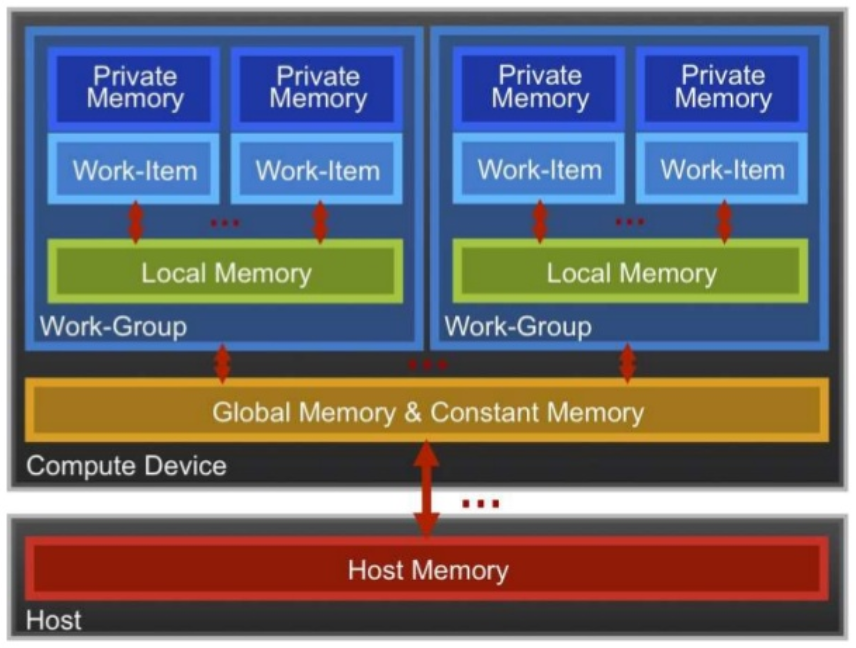
\includegraphics[width=125mm]{resources/opencl_hierarchy.png}
    \end{center}
    \caption{OpenCL memory hierarchy, source: \cite{opencl-hierarchy-diagram}.}
    \label{opencl-hierarchy}
\end{figure}

Hierarchical organization into NDRange, work-groups and work-items allows for more flexible mapping of computation tasks onto heterogeneous hardware
devices, which can have different architectures. Furthermore, it may also make it easier to map tasks onto OpenCL kernels. Complete tasks are defined
at the NDRange level, work-groups represent large computation chunks which are executed in arbitrary order. The smallest operations (e.g., addition of
two numbers) are mapped onto work-items.

Figure \ref{vector_addition} contains a simple OpenCL kernel, which performs addition of elements from arrays \textit{a} and \textit{b}, then stores
the result in array \textit{c}. Qualifier \textit{\_\_global} specified for the arguments means that they are stored in global memory. Function
\textit{get\_global\_id(int)} is used to retrieve work-item index unique for the entire NDRange in specified dimension.
\begin{figure}
\begin{lstlisting}
__kernel void vectorAddition(__global float* a, __global float* b, __global float* c)
{
    int i = get_global_id(0);
    c[i] = a[i] + b[i];
}
\end{lstlisting}
\caption{Vector addition in OpenCL.}
\label{vector_addition}
\end{figure}

\section{CUDA, comparison with OpenCL}
CUDA is a parallel compute API developed by Nvidia Corporation. It works similarly to OpenCL, but there are also several differences which played an
important role during the framework development:
\begin{itemize}
    \item CUDA is officially available only for graphics cards released by Nvidia Corporation and CPUs\footnote{PGI compiler provides CUDA support for CPUs.}.
    GPUs developed by other vendors and other types of accelerators are not supported.
    \item Differences in terminology -- identical or similar concepts have different terms in OpenCL and CUDA.
    \item Global indexing (i.e., NDRange indexing in OpenCL) works differently in CUDA.
\end{itemize}
Table \ref{api_terms} contains terms used in OpenCL and their counterparts in CUDA. Due to several differences in design, some terms do not have an
equivalent term in the other API.
\begin{table}[h]
\begin{center}
\begin{tabular}{|*{2}{p{5cm}|}}
    \hline
    OpenCL term & CUDA term \\
    \toprule
    compute unit & streaming multiprocessor \\
    processing element & CUDA core \\
    NDRange & grid \\
    work-group & thread block \\
    work-item & thread \\
    global memory & global memory \\
    constant memory & constant memory \\
    local memory & shared memory \\
    private memory & local memory \\
    cl\_platform & N/A \\
    cl\_device\_id & CUdevice \\
    cl\_context & CUcontext \\
    cl\_command\_queue & CUstream \\
    cl\_mem & CUdeviceptr \\
    cl\_program & nvrtcProgram, CUmodule \\
    cl\_kernel & CUfunction \\
    cl\_event & CUevent \\
    \hline
\end{tabular}
\end{center}
\caption{Comparison between OpenCL and CUDA terminology.}
\label{api_terms}
\end{table}

Difference in global indexing plays an important role during addition of tuning parameters which affect either grid dimensions or block dimensions.
In OpenCL, the NDRange size in a given dimension is specified as a size of work-group multiplied by number of work-groups. However, in CUDA the grid
size is specified only as a number of blocks. This is rather inconvenient for porting auto-tuned programs from one API to the other. The problem
will be further elaborated upon in Chapter \ref{ktt-api}.

\section{Possibilities for auto-tuning in compute APIs}
Design of previously described APIs allows for a wide range of optimization opportunities, both inside kernel and host code. These optimizations can
be implemented with usage of tuning parameters. While some of the parameters can be utilized only in a limited range of applications, there are also
several ones which are relevant for larger number of computation tasks. This section provides a list of some of the most common optimization parameters
which are used in code variant auto-tuning.

\subsection{Work-group (thread block) dimensions}
Work-group dimensions specify how many work-items are included in a single work-group. Work-groups are executed on compute units, which are mapped
onto, for example CPU cores or GPU multiprocessors. Performance of these devices may be vastly different and manually finding an optimal work-group
size in combination with other tuning parameters is difficult. The dimensions also indirectly affect cache locality of data, which is a reason why
this parameter usually makes an ideal candidate for auto-tuning.

\subsection{Usage of vector data types}
Modern processors contain vector registers that allow concurrent execution of a single instruction over multiple data which leads to a significant
speed-up of certain types of computations. Kernel compilers attempt to automatically utilize these registers in order to speed up computation without
manual code modification. However, automatic vectorization is not always optimal. There is an option to perform manual vectorization by using vector
data types which are available in both OpenCL and CUDA. It is possible to control vector length with a tuning parameter, e.g., by using type aliases.

\subsection{Data placement in different types of memory}
Section \ref{kernel} described various memory types available in OpenCL, similar memory hierarchy can also be found in CUDA. In many cases, there are
more valid memory types to choose from for data placement. The choice can have an effect on performance, for example accessing data from OpenCL local
memory is usually faster than using global memory. The problem is that local memory capacity is limited and while on certain devices the data could
fit into it, on other devices it would be necessary to use global memory instead. Having a single version of kernel which would utilize only global
memory would be inefficient for large number of devices. This can be solved by using tuning parameter which controls the data memory placement.

\subsection{Data layout in memory}
Composite data can be organized into memory in multiple ways. For example, data about 3D vertex coordinates can be split into three separate arrays
which are then stored in memory one by one. Another way to organize the same data is to first put all information about vertex into a structure and
then create an array of these structures. The former layout is commonly referred to as structure of arrays (SoA), while the latter is called array
of structures (AoS). The difference is illustrated with Figure \ref{aos_soa}.

The benefit of SoA is that variables with the same data type are stored in contiguous memory, which enables certain devices (e.g., Intel CPUs) to more
efficiently utilize vector instructions. Other types of devices such as GPUs support native vector addressing and usage of SoA layout may lead to
performance degradation.

\subsection{Combining multiple parameters}
In many situations, multiple tuning parameters can be utilized at once in order to further increase performance. However, certain parameters may affect
each other. For example, optimal work-group size can be different when data is stored in global memory compared to a situation where it is placed in
local memory. This makes it difficult to obtain the best combination manually, especially when many tuning parameters are used. Feasible solution is to
automatize this process.

\begin{figure}
\begin{lstlisting}
// 3D vertex coordinates stored as AoS and SoA.
struct                       struct
{                            {
    int x;                       int x[N];
    int y;                       int y[N];
    int z;                       int z[N];
} AoS[N];                    } SoA;
\end{lstlisting}
\caption{Comparison of array of structures and structure of arrays layouts.}
\label{aos_soa}
\end{figure}

\chapter{Code variant auto-tuning and related frameworks}
This chapter describes common terms used in relation to auto-tuning and provides a list of desired features which should be supported by auto-tuning
frameworks. Afterwards, several generic frameworks are presented, including their advantages, disadvantages, usage examples and comparison. Frameworks
which are domain-specific or not publicly available are not discussed here.

\section{Auto-tuning glossary}
The following terms are commonly encountered in subsequent chapters and their knowledge is required for better understanding of auto-tuning process:
\begin{itemize}
    \item \textit{tuning parameter} -- Parameter which, depending on its value, affects performance of a computation. For example, a parameter which
    controls length of a vector type of some variable. The exact way parameter comes into effect depends on a specific framework. Common option is
    utilization of just-in-time compilation and preprocessor macros.
    \item \textit{configuration space} -- Space which is created as a Cartesian product of all tuning parameters and their values. Certain elements of
    configuration space may be eliminated by utilizing constraints.
    \item \textit{tuning configuration} -- Single element of configuration space.
    \item \textit{traversal of configuration space} -- A process where tuned program is launched repeatedly with different tuning configurations and
    its running time is measured.
    \item \textit{search method} -- A method employed to explore individual tuning configurations. Because configuration space may become very large,
    exhaustive search is not always a viable option. It is possible to explore the space randomly or utilize an optimization method.
\end{itemize}

\section{Features of auto-tuning frameworks}
While there are no strict requirements over functionality that should be available in auto-tuning frameworks, there are several features which are either
commonly implemented by existing frameworks or desired by users. They include the following: 
\begin{itemize}
    \item Scope of tuning parameters -- While tuning parameters are supported by essentially all frameworks, not all of them allow parameters to affect
    all parts of a program. For example, some frameworks support only parameters which affect kernel code but not host code.
    \item Parameter constraints -- Ability to mark certain tuning configurations as invalid due to incompatible combinations of tuning parameter values.
    Such configurations should be excluded from configuration space traversal, which can lead to improved usability and performance.
    \item Advanced search methods -- Support for different methods which offer reasonable performance and quality of results.
    \item Output validation -- Certain tuning configurations might include code which is experimental or still in development. Tuner should offer
    an ability to compare the produced output with precomputed reference output and detect differences.
    \item Usage of kernel compositions -- A computation may utilize multiple kernels in order to produce complete result. The kernels may share some
    tuning parameters and a framework should be able to generate tuning configurations which support such scenarios.
    \item Online auto-tuning -- Ability to combine configuration space traversal with regular computation. Output from tested tuning configurations can
    be immediately utilized in other parts of a program. This is valuable in situations where tuning cannot be done prior to program execution, for
    example when optimal selection of tuning parameters depends on input.
    \item Integration into existing software -- Framework should not significantly restrict usage of features which are available in compute APIs.
    Ideally, users should be able to port native applications into framework without losing access to some of the corresponding compute API functionality.
    \item User-friendliness and ease of use -- Availability of documentation, tutorials, clean and stable API. Availability of utility methods such
    as printing of tuning results in common format, logging of debug information and others.
\end{itemize}

\section{CLTune}
CLTune \cite{cltune} is a framework for auto-tuning of OpenCL and CUDA kernels. It is freely available in form of a library and provides C++ interface
for writing host programs. It is relatively easy to use and provides capabilities for tuning of separate kernels, multiple configuration search
strategies including several optimization-based approaches and result validation in a form of reference kernels.

However, it also has several limitations. Among the most significant ones are lack of support for kernel compositions, limited argument handling
options (all kernels must accept the same kernel arguments, argument placement in memory is impossible to control) and poor support for integration into
existing software (code which launches kernels is internal part of the framework and cannot be modified). This results in a need to write separate
applications for tuning and computation. The framework is no longer actively developed, so it is unlikely that new features will be introduced.

Basic tuner configuration in CLTune consists of several main steps, which are listed below. KTT functionality, in its simplest form, is based on the
same idea. Figure \ref{cltune-example} contains part of a program written in CLTune, which includes all of the following steps:
\begin{enumerate}
    \item Initialization of tuner by specifying target platform and device.
    \item Addition of tuned kernel.
    \item Addition of reference kernel for output validation.
    \item Definition of tuning parameters.
    \item Setup of kernel arguments.
    \item Launch of the tuning process.
    \item Retrieval of results.
\end{enumerate}

\begin{figure}
\begin{adjustwidth}{-1cm}{-1cm}
\begin{lstlisting}
cltune::Tuner tuner(platformIndex, deviceIndex);
size_t kernelId = tuner.AddKernel({"path/to/kernel.cl"}, "kernelName", ndRangeDimensions, workGroupDimensions);
tuner.SetReference({"path/to/reference_kernel.cl"}, "referenceKernelName", ndRangeDimensions, workGroupDimensions);

tuner.AddParameter(kernelId, "VECTOR_TYPE", { 1, 2, 4, 8 });
tuner.AddParameter(kernelId, "USE_CONSTANT_MEMORY", { 0, 1 });

tuner.AddArgumentInput(bufferA);
tuner.AddArgumentInput(bufferB);
tuner.AddArgumentScalar(helperVariable);
tuner.AddArgumentOutput(bufferResult);

tuner.Tune();
tuner.PrintToScreen();
\end{lstlisting}
\caption{Host program written in CLTune.}
\label{cltune-example}
\end{adjustwidth}
\end{figure}

In order to support tuning parameters, kernel source file needs to be modified. In case of CLTune, the tuner exports parameter values from given
configuration to kernel source code by using preprocessor macros. Kernel code has to be modified by user, so that the exported values have intended
effect on computation. Simple example of such modification is shown in Figure \ref{cltune-example-kernel}.
\begin{figure}
\begin{lstlisting}
#if USE_CONSTANT_MEMORY == 0
#define MEMORY_TYPE __global
#elif USE_CONSTANT_MEMORY == 1
#define MEMORY_TYPE __constant
#endif

__kernel void tunedKernel(MEMORY_TYPE float* bufferA, ...)
{
    ...
}
\end{lstlisting}
\caption{Adding support for auto-tuning to kernel via preprocessor macros.}
\label{cltune-example-kernel}
\end{figure}

\section{Kernel Tuner}
Kernel Tuner \cite{kerneltuner} is another open-source auto-tuning framework. It supports tuning of OpenCL and CUDA kernels as well as regular C functions,
though in the last case, user is responsible for measuring execution duration. API is provided for Python. Compared to CLTune, it provides more utility
methods, for example ability to set kernel compiler options, measuring execution duration in multiple iterations to increase accuracy and validating output
with user-defined precomputed answer rather than being restricted to reference kernel.

As in case of CLTune, disadvantages include lack of support for kernel compositions and inability for integration into existing software. However,
Kernel Tuner is still actively developed and some of these shortcomings may be eventually amended.

Host program has to be written in similar fashion to CLTune, definitions of tuning parameters are exported in the same way. Figure \ref{kerneltuner-example}
contains major portion of host program written for Kernel Tuner.
\begin{figure}[ht]
\begin{adjustwidth}{-1cm}{-1cm}
\begin{lstlisting}
def tune():

with open('stencil.cl', 'r') as f:
kernel_string = f.read()

problem_size = (4096, 2048)
size = numpy.prod(problem_size)

x_old = numpy.random.randn(size).astype(numpy.float32)
x_new = numpy.copy(x_old)
args = [x_new, x_old]

tune_params = OrderedDict()
tune_params["block_size_x"] = [32*i for i in range(1,9)]
tune_params["block_size_y"] = [2**i for i in range(6)]

grid_div_x = ["block_size_x"]
grid_div_y = ["block_size_y"]

return kernel_tuner.tune_kernel("stencil_kernel", kernel_string, problem_size, args, tune_params, grid_div_x=grid_div_x, grid_div_y=grid_div_y)

if __name__ == "__main__":
    tune()
\end{lstlisting}
\caption{Host program written in Kernel Tuner, source: \cite{kerneltuner-example}.}
\label{kerneltuner-example}
\end{adjustwidth}
\end{figure}

\section{OpenTuner}
Unlike other mentioned tuners, OpenTuner \cite{opentuner} is an auto-tuning framework which can be used to tune programs written in essentially any
language. It supports multiple forms of auto-tuning, for example tuning of compiler flags or CPU frequencies as well as code variant auto-tuning. The
API is provided for Python. Due to tuner's more generic nature, users are responsible for writing more sections of code themselves. In case of code
variant auto-tuning, this involves writing a method which adds parameter definitions from tuner-generated configurations to tuned program and compiles
it. The other listed frameworks have this functionality already built-in. Other shortcomings include problems with integration into software and lack of
complete API documentation. Framework does not seem to be actively developed anymore with majority of the development being done before 2017.

While the other frameworks use preprocessor definitions to export tuning parameters into code, OpenTuner does not have any specific way of parameter
handling. The way parameters become visible in tuned code depends on capabilities of target programming language and on the user-written method for
parameter export. Figure \ref{opentuner-example} contains an example of OpenTuner configuration for tuning of C code. Tuning parameters are added
to code through compiler command line arguments.

\begin{figure}[ht]
\begin{adjustwidth}{-1cm}{-1cm}
\begin{lstlisting}
class GccFlagsTuner(MeasurementInterface):

def manipulator(self):
    manipulator = ConfigurationManipulator()
    manipulator.add_parameter(IntegerParameter('vectorType', 1, 2, 4, 8))
    return manipulator

def run(self, desired_result, input, limit):
    cfg = desired_result.configuration.data

gcc_cmd = 'g++ tuned_program.cpp '
gcc_cmd += '-VECTOR_TYPE='+ cfg['vectorType']
gcc_cmd += ' -o ./tmp.bin'

compile_result = self.call_program(gcc_cmd)
assert compile_result['returncode'] == 0

run_cmd = './tmp.bin'
run_result = self.call_program(run_cmd)
assert run_result['returncode'] == 0

return Result(time=run_result['time'])

def save_final_config(self, configuration):
    print "Optimal vector type written to final_config.json:", configuration.data
    self.manipulator().save_to_file(configuration.data, 'final_config.json')
\end{lstlisting}
\caption{Configuration of OpenTuner, source: \cite{opentuner}.}
\label{opentuner-example}
\end{adjustwidth}
\end{figure}

\section{ATF}
ATF (Auto-Tuning Framework) \cite{atf} is a recently released framework which offers several improvements over the previous solutions. Similarly to
OpenTuner, it supports several forms of auto-tuning and multiple languages. Unlike other mentioned frameworks, it relies on annotating user code
with directives and there is therefore no need to write separate tuning program. Another advantage is the ability to generate configuration space
more efficiently by utilizing multi-threading and pre-filtering of parameter values based on constraints. This improves tuner performance in
situations where many tuning parameters with large number of valid values are used.

ATF also supports various abort conditions to end exploration of search space during offline tuning. These include conditions based on absolute tuning
time, number of explored configurations and relative speedup within the last tested configurations. However, several shortcomings which were present
in previous frameworks also remain in ATF. There is no support for online tuning and no explicit support for kernel compositions. The framework currently
also lacks documentation and provides only a handful of usage examples. Another inconvenience is the necessity to ask for usage permission.

Example of tuning OpenCL SAXPY (single-precision a * x + y) kernel with ATF framework can be seen in Figure \ref{atf-example}.

\begin{figure}
\begin{adjustwidth}{-1cm}{-1cm}
\begin{lstlisting}
int main() {
const int N = 1024;

const ::std::string saxpy = R"cl__( 
__kernel void saxpy(const int N, const float a, const __global float* x, __global float* y)
{       
    for(int w = 0; w < WPT; ++w) {
        const int id = w * get_global_size(0) 
        + get_global_id(0);
        y[id] += a * x[id];
    }
}
)cl__";

auto WPT = atf::tp("WPT", atf::interval<int>(1, N), atf::divides(N));

auto LS = atf::tp("LS", atf::interval<int>(1, N), atf::divides(N / WPT));

auto cf_saxpy =
atf::cf::ocl({0, atf::cf::device_info::GPU, 1}, {saxpy, "saxpy"},
inputs(atf::scalar<int>(N),    // N
atf::scalar<float>(),   // a
atf::buffer<float>(N),  // x
atf::buffer<float>(N)), // y
atf::cf::GS(N / WPT), atf::cf::LS(LS));

auto best_config = atf::annealing(
atf::cond::duration<std::chrono::minutes>(2))(WPT, LS)(cf_saxpy);
}
\end{lstlisting}
\caption{Example of tuning SAXPY kernel with ATF, source: \cite{atf-example}.}
\label{atf-example}
\end{adjustwidth}
\end{figure}

\section{Comparison of frameworks}
Table \ref{frameworks-comparison} showcases state of features in previously discussed frameworks. Note that state of the supported features may change
as several mentioned frameworks are still actively developed.

\begin{sidewaysfigure}[ht]
\begin{adjustwidth}{-3cm}{-1cm}
\begin{tabular}{|L{4cm}L{4cm}L{4cm}L{4cm}L{4cm}|}
\hline
\multicolumn{1}{|c}{\textbf{Feature}} & \multicolumn{1}{c}{\textbf{CLTune}} & \multicolumn{1}{c}{\textbf{Kernel Tuner}} & \multicolumn{1}{c}{\textbf{OpenTuner}} & \multicolumn{1}{c|}{\textbf{ATF}} \\
\hline
Supported APIs & CUDA, OpenCL & CUDA, OpenCL & any language or API & any language or API \\
Tuning parameters & kernel code only & kernel and host code & kernel and host code & kernel and host code \\
Parameter constraints & \multicolumn{1}{c}{\checkmark} & \multicolumn{1}{c}{\checkmark} & requires additional user effort & \multicolumn{1}{c|}{\checkmark} \\
Search methods & multiple optimization methods supported & multiple optimization methods supported & multiple optimization methods supported & multiple optimization methods supported \\
Output validation & reference kernel only & reference kernel or precomputed buffer & \multicolumn{1}{c}{X} & \multicolumn{1}{c|}{X} \\
Kernel compositions & \multicolumn{1}{c}{X} & \multicolumn{1}{c}{X} & requires additional user effort & \multicolumn{1}{c|}{X} \\
Online auto-tuning & \multicolumn{1}{c}{X} & \multicolumn{1}{c}{X} & \multicolumn{1}{c}{X} & \multicolumn{1}{c|}{X} \\
Full API documentation & \multicolumn{1}{c}{\checkmark} & \multicolumn{1}{c}{\checkmark} & \multicolumn{1}{c}{X} & \multicolumn{1}{c|}{X} \\
\hline
\end{tabular}
\caption{Comparison of features in auto-tuning frameworks.}
\label{frameworks-comparison}
\end{adjustwidth}
\end{sidewaysfigure}

\FloatBarrier

\chapter{KTT framework}
\label{ktt-api}

While the previously mentioned frameworks handle auto-tuning of single kernels well and provide fairly wide range of utility methods, they all lack
support for tuning of kernel compositions and online auto-tuning. They were designed for tuning of separate programs combined with explicit exporting
of optimized parameter values into production code without possibility of integration into existing software. These are the main features which should
be included in the new auto-tuning framework.

Originally, CLTune was planned to be used as a basis for the new framework. Extra functionality was to be added on top of the existing code structure.
However, this has proved to be rather problematic. While CLTune API is written in a clean and user-friendly manner, its internal structure made it
difficult to extend its functionality. Large part of the internal code is placed into a small number of very long methods which mix together operations
such as argument handling and result validation with access to compute API functions. This made it difficult to introduce new features without refactoring
large amount of code.

Eventually, it was decided to write a completely new framework named Kernel Tuning Toolkit. Baseline portion of KTT API remained similar to CLTune,
so it would be easy to port existing programs. However, the internal structure was completely rewritten from scratch, with only very small portions
of CLTune code for following features being reused:
\begin{itemize}
    \item generating of tuning configurations
    \item definition of tuning parameter constraints
    \item search methods based on simulated annealing and particle swarm optimization techniques
\end{itemize}
The new tuner structure is further discussed in chapter \ref{ktt-structure}.

\section{Overview of KTT functionality}
This section describes different usage scenarios supported by KTT framework and provides a high-level overview of the steps performed in each scenario.

\subsection{Single kernel tuning}
The simplest scenario which is also supported by all of the previously discussed frameworks is offline tuning of a single kernel. The tuning process in
this case is similar to that of CLTune framework. Addition of tuned kernel and its arguments to tuner is followed by definition of tuning parameters.
Framework then performs the tuning, including handling of kernel execution and buffer management. Tuning results are reported once the operation is
finished. The entire workflow is illustrated in Figure \ref{ktt-sequence-diagram-single}. A concrete example of this usage scenario is described in
Section \ref{ktt-simple-usage}.

\subsection{Kernel compositions and host code tuning}
A more complex situation is tuning of a computation which involves execution of multiple kernels and performs portion of a computation on a CPU (e.g.,
output from one kernel organized in structure of arrays layout is transformed in a CPU code into array of structures layout and then used as input for
other kernel). Solution provided by KTT framework for such scenarios is called tuning manipulator, which enables users to customize portion of the
framework's code that is responsible for kernel execution and buffer management, and optionally perform some part of computation directly in C++ code.
The general usage is shown in Figure \ref{ktt-sequence-diagram-composite}. Further information about manipulators can be found in Section
\ref{ktt-manipulator}. Specific examples utilizing kernel compositions and tuning manipulators are located in Chapter \ref{ktt-advanced-usage}.

\subsection{Online tuning and software integration}
The two previous sections described situations involving tuning of standalone computations. However, KTT framework also supports integration into other
applications. There are two possible usage scenarios:
\begin{itemize}
    \item Tuning is performed at the start of application, which can then transparently continue its computation. Tuning is integrated directly with
    the application and there is no need for separate tuning program.
    \item Tuning is performed at the time of computation. Application executes kernels and uses their output while KTT transparently changes tuning
    parameters and searches for the best configuration. This scenario is referred to as online tuning and is beneficial in cases when kernel running
    time dominates over tuning overhead as all of the kernel executions contribute to final result. An example of this way of usage is in Chapter
    \ref{ktt-advanced-usage}.
\end{itemize}

\clearpage
\thispagestyle{plain}
\begin{sidewaysfigure}
    \begin{adjustwidth}{-3.5cm}{-3.5cm}
        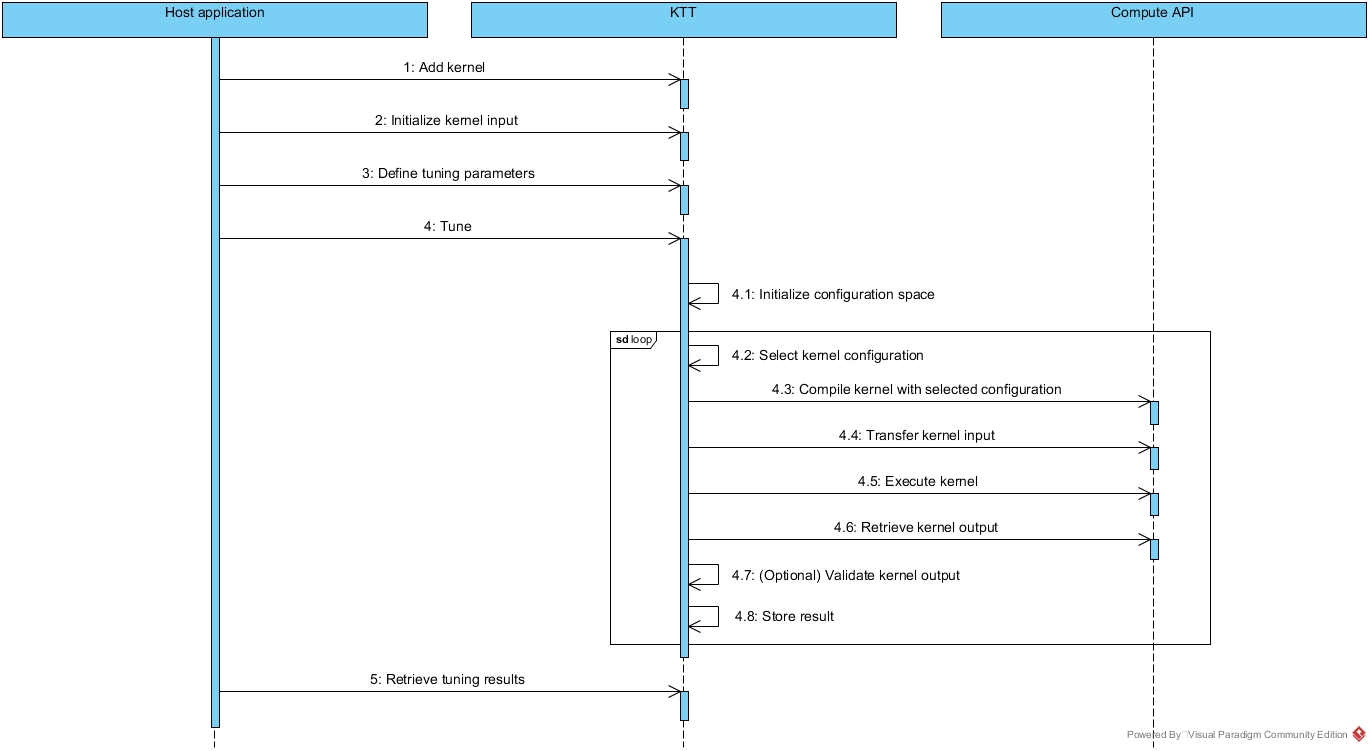
\includegraphics[width=250mm]{resources/ktt_sequence_diagram_single.jpg}
    \end{adjustwidth}
    \caption{Diagram showcasing offline tuning of a single kernel.}
    \label{ktt-sequence-diagram-single}
\end{sidewaysfigure}
\clearpage

\clearpage
\thispagestyle{plain}
\begin{sidewaysfigure}
    \begin{adjustwidth}{-3.5cm}{-3.5cm}
        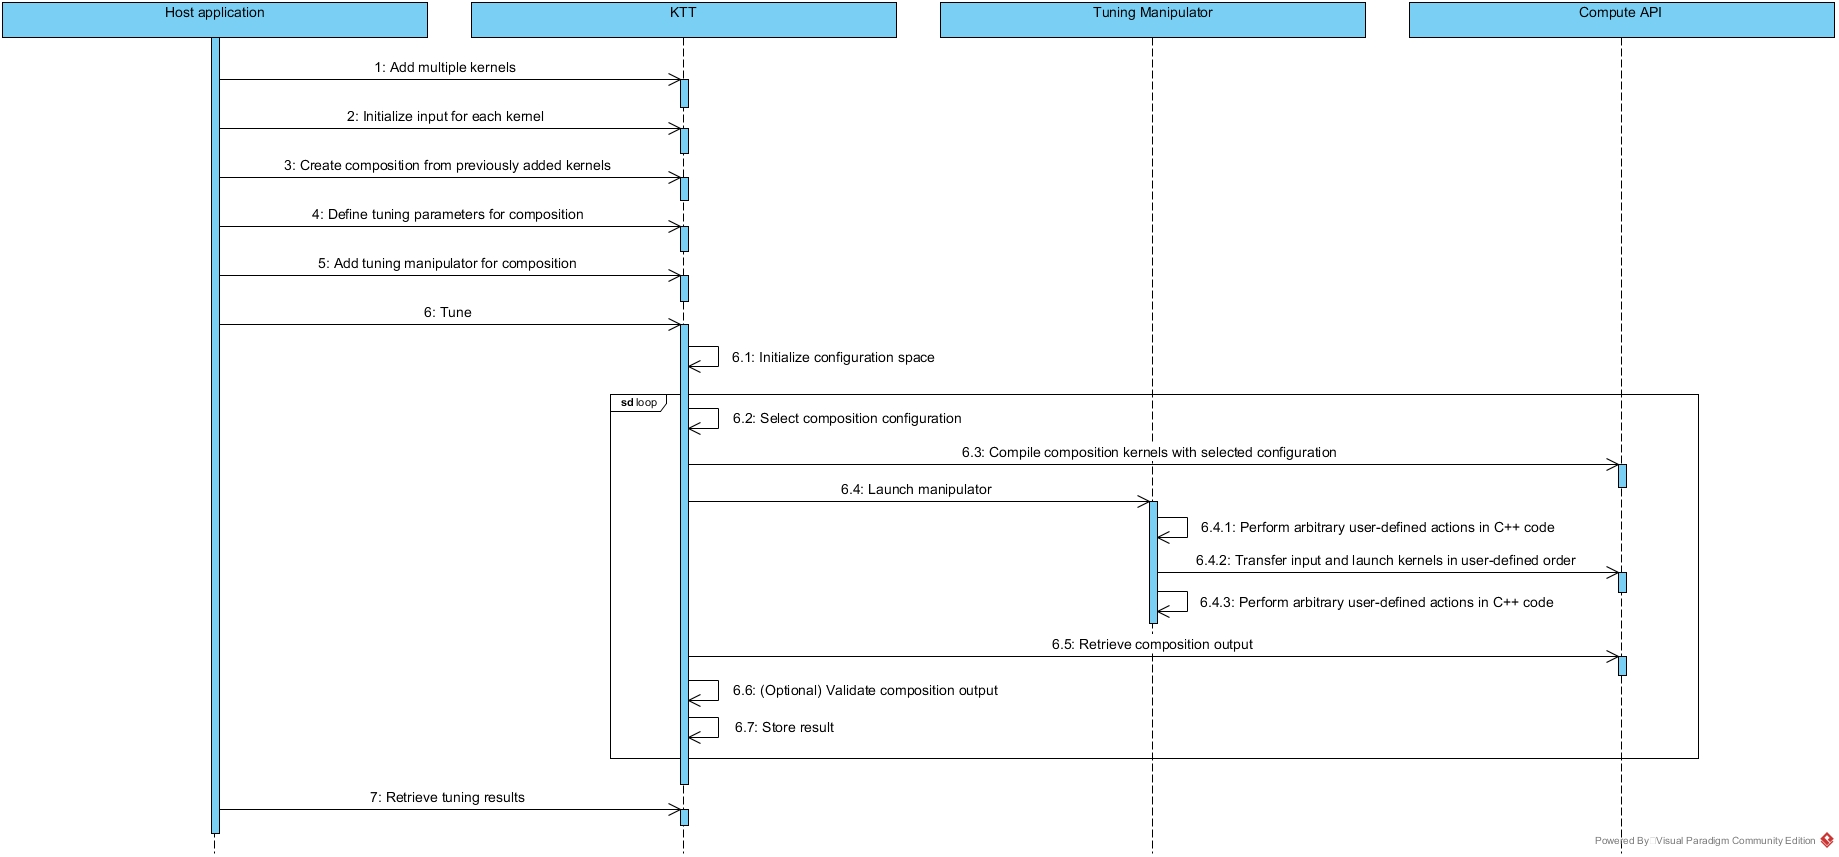
\includegraphics[width=250mm]{resources/ktt_sequence_diagram_composite.jpg}
    \end{adjustwidth}
    \caption{Diagram showcasing offline tuning of a kernel composition utilizing tuning manipulator.}
    \label{ktt-sequence-diagram-composite}
\end{sidewaysfigure}
\clearpage

\section{KTT API}
KTT framework API provides users with methods which can be used to develop and tune OpenCL or CUDA applications. It is split into three major
classes, some basic methods were inspired by CLTune. It is written in C++ language.

KTT framework can be acquired from GitHub as a fully open-source library with prebuilt binaries being available for certain platforms. Manual library
compilation is also possible by using build tool premake5, C++14 compiler and CUDA or OpenCL distribution. Supported operating systems include Linux
and Windows.

The described API corresponds to version 0.6 of KTT framework. It is the first release candidate version and contains all functionality that was
planned to be implemented as part of this thesis.

\section{Tuner class}
Tuner class makes up the main part of KTT API. It includes methods which implement following functionality:
\begin{itemize}
    \item handling of kernels and kernel compositions
    \item handling of kernel arguments
    \item addition of tuning parameters and constraints
    \item kernel running and tuning
    \item kernel output validation
    \item retrieval of tuning results
    \item retrieval of information about available platforms and devices
\end{itemize}

\subsection{Tuner creation}
In order to access the API methods, tuner object has to be created. There are currently three versions of tuner constructors available (Figure 
\ref{ktt-constructors}). They allow specification of compute API (either OpenCL or CUDA), platform index, device index and number of utilized compute
queues. OpenCL API with one compute queue is the default setting. Indices are assigned to platforms and devices by KTT framework, they can be retrieved
with a method.

\begin{figure}
\begin{adjustwidth}{-1cm}{-1cm}
\begin{lstlisting}
Tuner(const PlatformIndex platform, const DeviceIndex device)
Tuner(const PlatformIndex platform, const DeviceIndex device, const ComputeAPI API)
Tuner(const PlatformIndex platform, const DeviceIndex device, const ComputeAPI API, const uint32_t computeQueueCount)
\end{lstlisting}
\caption{Tuner constructors.}
\label{ktt-constructors}
\end{adjustwidth}
\end{figure}

\subsection{Kernel handling}
Kernels can be added to a tuner from a file or C++ string (Figure \ref{ktt-kernel-methods}). Users furthermore need to specify kernel function name and
default global and local sizes (i.e., dimensions for NDRange / grid and work-group / thread block). The sizes are stored inside \textit{DimensionVector}
objects, which are a part of KTT framework. They allow easy thread size manipulation and support up to three dimensions. Existing kernels can be referenced
by using a handle returned by tuner. Kernel compositions can be added by specifying handles of kernels included inside a composition. In order to use
compositions, user additionally has to define a tuning manipulator class whose usage is detailed in Section \ref{ktt-manipulator}.

\begin{figure}
\begin{adjustwidth}{-1cm}{-1cm}
\begin{lstlisting}
KernelId addKernel(const std::string& source, const std::string& kernelName, const DimensionVector& globalSize, const DimensionVector& localSize)
KernelId addKernelFromFile(const std::string& filePath, const std::string& kernelName, const DimensionVector& globalSize, const DimensionVector& localSize)
KernelId addComposition(const std::string& compositionName, const std::vector<KernelId>& kernelIds, std::unique_ptr<TuningManipulator> manipulator)
\end{lstlisting}
\caption{Kernel addition methods.}
\label{ktt-kernel-methods}
\end{adjustwidth}
\end{figure}

\subsection{Kernel argument handling}
There are three types of kernel arguments supported by KTT -- vector, scalar and local memory (OpenCL) arguments. All arguments are referenced by using
a handle provided by a tuner. Argument addition methods are templated and support primitive data types (e.g., int, float) as well as user-defined data
types (e.g., struct, class). Arguments are bound to kernels by using a method which accepts kernel handle and corresponding argument handles. This allows
them to be shared among multiple kernels. The mentioned methods can be seen in Figure \ref{ktt-argument-methods}.

Vector arguments are added from C++ vector containers. It is possible to specify access type (read, write or combined), memory location from where
argument data is accessed by kernel (device or host) and whether argument copy should be made by tuner. By default, copies of all vector arguments
are made by tuner, so the original vectors remain modifiable by user without interfering with tuning process. In case argument is placed in host
memory, it is possible to utilize zero-copy feature, which means that kernel has direct access to buffer which was initialized from host code. This
functionality is supported by both CUDA and OpenCL. All of the vector argument handling options are illustrated with Figure \ref{ktt-buffer-diagram}.

\begin{figure}
\begin{adjustwidth}{-1cm}{-1cm}
\begin{lstlisting}
ArgumentId addArgumentVector(const std::vector<T>& data, const ArgumentAccessType accessType)
ArgumentId addArgumentVector(std::vector<T>& data, const ArgumentAccessType accessType, const ArgumentMemoryLocation location, const bool copyData)
ArgumentId addArgumentScalar(const T& data)
ArgumentId addArgumentLocal(const size_t localMemoryElementsCount)
void setKernelArguments(const KernelId id, const std::vector<ArgumentId>& argumentIds)
\end{lstlisting}
\caption{Argument handling methods.}
\label{ktt-argument-methods}
\end{adjustwidth}
\end{figure}

\begin{figure}
\begin{center}
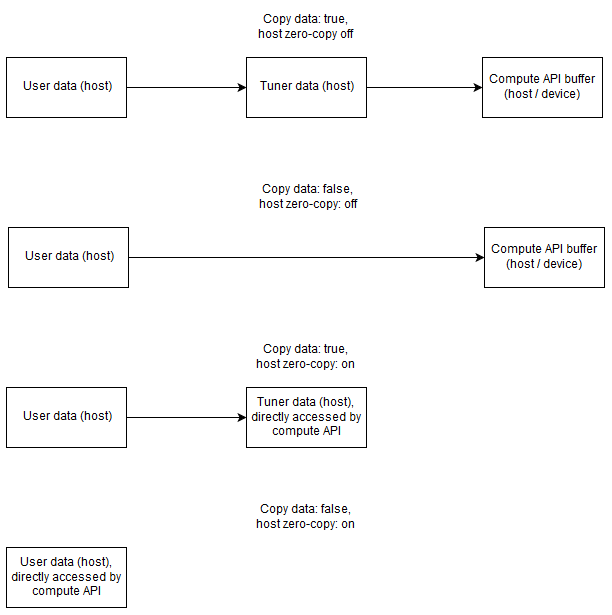
\includegraphics[width=125mm]{resources/ktt_buffer_diagram.png}
\end{center}
\caption{Vector argument handling options in KTT framework. Each box represents one copy of a buffer.}
\label{ktt-buffer-diagram}
\end{figure}

\subsection{Tuning parameters and constraints}
\label{ktt-tuning-parameters}
Tuning parameters are specified for kernels with a name and list of valid values (Figure \ref{ktt-parameter-methods}). Both integer and floating-point
values are supported. Before kernel tuning begins, configurations for each combination of kernel parameter values are generated. For example, adding
parameter A with values 1 and 2, and parameter B with values 5 and 10 will result in four configurations being generated -- \{1, 5\}, \{1, 10\}, \{2, 5\}
and \{2, 10\}. Tuned kernel is then launched with parameter definitions prepended to kernel source code based on the current configuration.

Some tuning parameters may additionally affect global and local sizes of tuned kernel. This is useful, for example, in cases where parameter in kernel
source code modifies amount of work done by a single work-item and therefore changes total number of needed work-items. Each dimension can be modified
separately, supported modifiers include addition, subtraction, multiplication and division.

If certain combinations of tuning parameters are invalid or unsupported by a kernel source code, they can be eliminated by using parameter constraints.
Constraint is a function which accepts list of parameter values for specified parameters and returns a boolean result which signifies whether the
combination is valid or not. Constraint conditions are defined by user.

Tuning parameters for kernel compositions are added separately and are shared by all kernels inside a composition. Individual kernels outside compositions
are not affected by composition parameters either.

\begin{figure}
\begin{adjustwidth}{-1cm}{-1cm}
\begin{lstlisting}
void addParameter(const KernelId id, const std::string& parameterName, const std::vector<size_t>& parameterValues)
void addParameterDouble(const KernelId id, const std::string& parameterName, const std::vector<double>& parameterValues)
void addParameter(const KernelId id, const std::string& parameterName, const std::vector<size_t>& parameterValues, const ModifierType type, const ModifierAction action, const ModifierDimension dimension)
void addConstraint(const KernelId id, const std::function<bool(std::vector<size_t>)>& constraintFunction, const std::vector<std::string>& parameterNames)
\end{lstlisting}
\caption{Tuning parameter and constraint addition methods.}
\label{ktt-parameter-methods}
\end{adjustwidth}
\end{figure}

\subsection{Kernel tuning and running}
KTT supports offline and online kernel tuning as well as regular kernel running. In offline tuning, kernel configurations are tested iteratively one
after another without interruption. This mode is strictly focused on finding the best performing configuration, retrieval of kernel output by user and
swapping of kernel argument data between configurations is not possible. On the other hand, it allows efficient validation of output. Because the
argument data remains the same for all configurations, the reference output needs to be computed only once.

In online tuning, single configuration is tested at time, enabling combination with kernel running. It also allows kernel output retrieval using
KTT built-in structure \textit{OutputDescriptor}. This structure specifies handle of argument to be retrieved, memory location for output data and
optionally size of the retrieved data, which is useful in case only part of the argument is needed. Online tuning also enables swapping of argument
data between each configuration, though if validation is enabled, reference output needs to be recomputed every time a new configuration is run.
It is important to note that the input size should remain the same across all tested configurations during tuning so that the measured durations
can be objectively compared. The optimal configurations are not necessarily identical for different input sizes either.

In both modes, the order and number of tested configurations depends on utilized search method. KTT currently supports five search methods -- full
search, random search, simulated annealing, particle swarm optimization and Markov chain Monte Carlo. Full search simply explores all configurations
iteratively. The other four methods allow specification of a fraction parameter which controls number of explored configurations (e.g., setting fraction
to 0.5 will result in 50\% of all configurations being tested). In random search, the explored configurations are chosen randomly, while the last three
methods employ probabilistic techniques in order to find configurations with good performance more quickly.

Output retrieval is supported for kernel running in the same fashion as for online tuning. Kernels can be run in any valid tuning configuration which is
specified by user. Output validation is not performed during kernel running. Kernels can be run using the best found configuration immediately after the
tuning finishes so that splitting auto-tuning and production applications is not necessary.

In basic case, launch of a kernel is handled automatically by a tuner after the initial setup. However, for scenarios where part of a computation
happens in C++ code or kernel compositions are utilized, it is necessary to implement a \textit{TuningManipulator} and then bind it to corresponding
kernel. Tuning manipulators are discussed in greater detail in Section \ref{ktt-manipulator}.

Figure \ref{ktt-tuning-methods} contains all of the previously described methods related to kernel tuning and running.

\begin{figure}
\begin{adjustwidth}{-1cm}{-1cm}
\begin{lstlisting}
void tuneKernel(const KernelId id)
void tuneKernelByStep(const KernelId id, const std::vector<OutputDescriptor>& output)
void runKernel(const KernelId id, const std::vector<ParameterPair>& configuration, const std::vector<OutputDescriptor>& output)
void setSearchMethod(const SearchMethod method, const std::vector<double>& arguments)
void setTuningManipulator(const KernelId id, std::unique_ptr<TuningManipulator> manipulator)
\end{lstlisting}
\caption{Kernel tuning and running methods.}
\label{ktt-tuning-methods}
\end{adjustwidth}
\end{figure}

\subsection{Output validation}
\label{ktt-validation}
Kernel output can be validated in two ways -- with a reference class or a reference kernel (Figure \ref{ktt-validation-methods}). In the former case,
user has to implement a class which includes a method that computes reference output on a CPU. Tuner then compares this output with result produced
by tuned kernels. If difference in tuned output at certain index is detected, given kernel configuration is considered invalid. More details about
reference class can be found in Section \ref{ktt-reference-class}. The latter case works similarly, difference being that reference output is computed
by a kernel with user-specified configuration. Both methods support validation of multiple kernel arguments. It is also possible to only check subpart
of the argument, which is useful when result is shorter than length of an entire argument.

When kernel arguments with floating-point data type are validated, user can choose one of the multiple validation techniques and a tolerance threshold.
If tuned output differs slightly from reference output, but remains within the threshold, it is still considered correct. Validation techniques include
side by side comparison where result difference is calculated and compared to threshold for each pair of elements with corresponding index in reference
and tuned output. Other technique is absolute difference, where the differences between individual pairs are summed up and only the resulting sum is
compared to threshold.

Users additionally have an option to add a custom comparator for specified argument. Comparator is a method which receives two elements with the same
data type and decides whether they are equal. Comparators are mandatory for arguments with user-defined data types as the tuner is only able to
automatically validate arguments with built-in data types.

\begin{figure}
\begin{adjustwidth}{-1cm}{-1cm}
\begin{lstlisting}
void setReferenceKernel(const KernelId id, const KernelId referenceId, const std::vector<ParameterPair>& referenceConfiguration, const std::vector<ArgumentId>& validatedArgumentIds)
void setReferenceClass(const KernelId id, std::unique_ptr<ReferenceClass> referenceClass, const std::vector<ArgumentId>& validatedArgumentIds)
void setValidationMethod(const ValidationMethod method, const double toleranceThreshold)
void setValidationRange(const ArgumentId id, const size_t range)
void setArgumentComparator(const ArgumentId id, const std::function<bool(const void*, const void*)>& comparator)
\end{lstlisting}
\caption{Output validation methods.}
\label{ktt-validation-methods}
\end{adjustwidth}
\end{figure}

\subsection{Tuning results retrieval}
Each tuning result includes list of parameter values, global and local thread sizes and corresponding duration of computation. List of all tuning
results for specified kernel can be printed either to a C++ output stream or a file. Supported print formats include verbose format intended for log
files or terminals and CSV (comma-separated values) format which is useful for subsequent processing and analysis of results.

List of parameter values for the best known configuration can also be retrieved through an API method, which is useful for combining online
auto-tuning with kernel running. The available methods can be seen in figure \ref{ktt-result-methods}.

\begin{figure}
\begin{adjustwidth}{-1cm}{-1cm}
\begin{lstlisting}
void printResult(const KernelId id, std::ostream& outputTarget, const PrintFormat format)
void printResult(const KernelId id, const std::string& filePath, const PrintFormat format)
std::vector<ParameterPair> getBestConfiguration(const KernelId id)
\end{lstlisting}
\caption{Result retrieval methods.}
\label{ktt-result-methods}
\end{adjustwidth}
\end{figure}

\subsection{Platform and device information retrieval}
When using KTT framework for the first time on a system, it is useful to retrieve indices for available platforms and devices, which are then used for
proper tuner initialization. The assigned indices and corresponding platform and device names can be printed to specified C++ output stream. It is
furthermore possible to retrieve more detailed information about individual platforms and devices, such as list of supported extensions, memory
capacities, number of compute units and others (Figure \ref{ktt-information-methods}).

\begin{figure}
\begin{adjustwidth}{-1cm}{-1cm}
\begin{lstlisting}
void printComputeAPIInfo(std::ostream& outputTarget)
std::vector<PlatformInfo> getPlatformInfo()
std::vector<DeviceInfo> getDeviceInfo(const PlatformIndex index)
DeviceInfo getCurrentDeviceInfo()
\end{lstlisting}
\caption{Information retrieval methods.}
\label{ktt-information-methods}
\end{adjustwidth}
\end{figure}

\subsection{Other notable methods}
Other notable API methods include a method for specification of kernel compiler options, choice of a global size notation and an option to enable
automatic global size correction (Figure \ref{ktt-utility-methods}). Compiler options can be specified as a string of individual flags separated by
a white space.

Choice of a global size notation allows using OpenCL NDRange dimension specification for CUDA grid and vice versa. This allows elimination of one of
the notable differences between OpenCL and CUDA API in host code and makes it easier to port programs written in one API to the other.

Automatic global size correction ensures that global size is always a multiple of local size, which is a necessary requirement for running kernels
in OpenCL, and also in CUDA if OpenCL global size notation option is used. Framework performs automatic roundup of a global size to the nearest higher
multiple of a local size. Enabling this behaviour is useful when multiple tuning parameters which affect thread sizes are present.

\begin{figure}
\begin{adjustwidth}{-1cm}{-1cm}
\begin{lstlisting}
void setCompilerOptions(const std::string& options)
void setGlobalSizeType(const GlobalSizeType type)
void setAutomaticGlobalSizeCorrection(const bool flag)
\end{lstlisting}
\caption{Other notable methods.}
\label{ktt-utility-methods}
\end{adjustwidth}
\end{figure}

\section{Reference class}
\label{ktt-reference-class}
Reference class is an interface provided by KTT framework used for validating of kernel output via implementing a C++ function. In order to utilize it,
a new class which publicly inherits from \textit{ReferenceClass} interface must be defined by a user. For the resulting class to be valid, it is
necessary to implement two virtual methods and optionally override one more method (Figure \ref{ktt-reference-methods}).

The first method should implement computation of a reference output. The second method is then used to retrieve the prepared output. The third, optional
method can be overriden if the resulting output size is smaller than the size of corresponding validated kernel argument. This is useful for situations
where only a part of the argument is validated.

Implemented class can be then assigned to a tuner by using a method from tuner API described in Section \ref{ktt-validation}. The implemented
methods are utilized by a tuner during output validation phase.

\begin{figure}
\begin{adjustwidth}{-1cm}{-1cm}
\begin{lstlisting}
virtual void computeResult() = 0
virtual void* getData(const ArgumentId id) = 0
virtual size_t getNumberOfElements(const ArgumentId id)
\end{lstlisting}
\caption{Reference class methods.}
\label{ktt-reference-methods}
\end{adjustwidth}
\end{figure}

\section{Tuning manipulator class}
\label{ktt-manipulator}
Tuning manipulator is an interface for customizing the way kernels are launched inside KTT framework. This is useful in several scenarios:
\begin{itemize}
    \item Tuned kernel is launched iteratively in order to produce complete result.
    \item Part of a computation happens on a CPU side in C++ code.
    \item Tuning parameters which affect host code are present.
    \item Kernel compositions are utilized.
    \item Framework is integrated into another software which needs to perform additional operations between individual kernel launches.
\end{itemize}

Because in all of the above-mentioned scenarios, the exact way kernel is launched depends on a specific use case, it is up to user to define their own
tuning manipulator. The definition works in a similar way as for reference class -- a new class inheriting from \textit{TuningManipulator} interface
has to be created and a virtual method which launches a kernel and performs any user-defined operations needs to be implemented.

Tuning manipulator interface also includes several other methods which can be used by a user within the kernel launch method. These include methods
for work with multiple compute queues, asynchronous operations, buffer management and methods which make handling of tuning parameters affecting
host code easier.

\subsection{Kernel running and host code tuning}
The basic task which needs to be fulfilled by the implemented method is to run a kernel with corresponding tuning configuration. If the implemented
method executes only this one task, then the resulting behaviour is the same as if no tuning manipulator was used at all.

Kernel in tuning manipulator can be run either with global and local thread sizes corresponding to current configuration or with user-specified sizes.
Second option can be used in addition or as an alternative to thread size modifying parameters described in Section \ref{ktt-tuning-parameters}.
Methods for thread size and parameter value retrieval are available as well. Those can be used to implement tuning parameters which affect host code.
The list of all tuning manipulator methods related to kernel running can be seen in Figure \ref{ktt-manipulator-kernel-methods}.

\begin{figure}
\begin{adjustwidth}{-1cm}{-1cm}
\begin{lstlisting}
void runKernel(const KernelId id)
void runKernel(const KernelId id, const DimensionVector& globalSize, const DimensionVector& localSize)
DimensionVector getCurrentGlobalSize(const KernelId id)
DimensionVector getCurrentLocalSize(const KernelId id)
std::vector<ParameterPair> getCurrentConfiguration()
\end{lstlisting}
\caption{Kernel running and configuration retrieval methods.}
\label{ktt-manipulator-kernel-methods}
\end{adjustwidth}
\end{figure}

\subsection{Kernel argument and buffer management}
When a kernel is run iteratively to produce complete result, it is often desirable to modify the input data between iterations. Tuning manipulator
interface provides methods for this scenario. It is possible to modify both scalar and vector arguments. It is also possible to retrieve data of
vector arguments, which is useful, for example when the data has to be preprocessed on a CPU in-between iterative kernel launches (Figure
\ref{ktt-manipulator-buffer-methods}).

All of the modifications performed on kernel arguments and corresponding buffers are isolated to a single tuning manipulator instance call. This makes
it possible to utilize manipulators in offline tuning, where the initial state of kernel arguments before testing of each tuning configuration needs to
remain the same.

\begin{figure}
\begin{adjustwidth}{-1cm}{-1cm}
\begin{lstlisting}
void updateArgumentScalar(const ArgumentId id, const void* argumentData)
void updateArgumentVector(const ArgumentId id, const void* argumentData, const size_t numberOfElements)
void getArgumentVector(const ArgumentId id, void* destination, const size_t numberOfElements)
void copyArgumentVector(const ArgumentId destination, const ArgumentId source, const size_t numberOfElements)
void changeKernelArguments(const KernelId id, const std::vector<ArgumentId>& argumentIds)
\end{lstlisting}
\caption{Kernel argument and buffer handling methods.}
\label{ktt-manipulator-buffer-methods}
\end{adjustwidth}
\end{figure}

\subsection{Compute queues and asynchronous operations}
In real-world computations, multiple compute queues are often utilized in order to overlap independent parts of a computation and thus increase
performance. For this purpose, manipulator interface includes methods for executing asynchronous operations in specified queue and device synchronization.
Number of queues which are available corresponds to user-specified amount during tuner initialization. Queues are referenced with handles provided by KTT.
Methods which can be run asynchronously include kernel running and operations with vector kernel arguments. It is possible to synchronize either only
specified queue or all queues which effectively synchronizes the entire device (Figure \ref{ktt-manipulator-asynchronous-methods}).

\begin{figure}
\begin{adjustwidth}{-1cm}{-1cm}
\begin{lstlisting}
QueueId getDefaultDeviceQueue()
std::vector<QueueId> getAllDeviceQueues()
void synchronizeQueue(const QueueId queue)
void synchronizeDevice()
void runKernelAsync(const KernelId id, const DimensionVector& globalSize, const DimensionVector& localSize, const QueueId queue)
void updateArgumentVectorAsync(const ArgumentId id, const void* argumentData, const size_t numberOfElements, QueueId queue)
\end{lstlisting}
\caption{Compute queue handling and asynchronous methods.}
\label{ktt-manipulator-asynchronous-methods}
\end{adjustwidth}
\end{figure}

\section{Example of API usage}
\label{ktt-simple-usage}
Figures \ref{ktt-api-usage-reference} and \ref{ktt-api-usage} contain a simple example of using KTT to tune OpenCL vector addition kernel (shown in
Figure \ref{vector_addition}).

Output validation is done via reference class interface which is defined in the first figure. User-defined constructor (lines 4-9) initializes all
the data that is needed to compute reference result. Method which computes the result (lines 11-17) performs a simple addition of elements inside
two vector containers in a for loop. The final method (lines 19-26) is called internally by KTT framework to retrieve computed reference result.
Since KTT validation component works directly with computed data, the method needs to return pointer to a buffer which contains this data rather than
pointer to the entire vector container. Because it is possible to validate multiple arguments with single reference class, this function also checks
for which argument the reference result should be returned.

Second figure then shows the main part of a host program. In this example, a kernel is tuned using single tuning parameter which controls size of a
work-group -- four possible parameter values are specified. Lines 5-16 contain initialization of data, global and local sizes. NDRange size is
initialized to total number of elements inside vector so that each element is processed by a single work-item. For simplicity's sake, it is assumed that
number of elements is a multiple of 32. Work-group size is initialized to one because it will be controlled with tuning parameter which is added later.
Tuner is initialized (line 18) by specifying platform and device index, followed by addition of tuned kernel and its arguments (lines 19-24). The next
line includes instantiation of previously defined reference class and its addition to tuner. Line 28 contains definition of a tuning parameter which
multiplies work-group size in dimension x. Since the default size was defined as 1, this effectively sets the resulting size to this parameter value.
Once all the configuration is done, tuning of kernel can be started (line 29) and is followed by printing of results to standard output stream (line 30).

More complex examples, including usage of tuning manipulator interface are covered in Chapter \ref{ktt-advanced-usage}.

\begin{figure}
\footnotesize
\begin{adjustwidth}{-1cm}{-1cm}
\begin{lstlisting}
class SimpleValidator : public ktt::ReferenceClass
{
public:
    SimpleValidator(const ktt::ArgumentId validatedArgument, const std::vector<float>& a, const std::vector<float>& b, const std::vector<float>& result) :
        validatedArgument(validatedArgument),
        a(a),
        b(b),
        result(result)
    {}
    
    void computeResult() override
    {
        for (size_t i = 0; i < result.size(); i++)
        {
            result.at(i) = a.at(i) + b.at(i);
        }
    }
    
    void* getData(const ktt::ArgumentId id) override
    {
        if (validatedArgument == id)
        {
            return result.data();
        }
        return nullptr;
    }
    
private:
    ktt::ArgumentId validatedArgument;
    const std::vector<float>& a;
    const std::vector<float>& b;
    std::vector<float> result;
};
\end{lstlisting}
\caption{KTT usage example -- reference class definition.}
\label{ktt-api-usage-reference}
\end{adjustwidth}
\end{figure}

\begin{figure}
\footnotesize
\begin{adjustwidth}{-1cm}{-1cm}
\begin{lstlisting}
int main(int argc, char** argv)
{
    // Initialize platform / device index and path to kernel file.
    ...
    const size_t numberOfElements = 1024 * 1024;
    const ktt::DimensionVector ndRangeDimensions(numberOfElements);
    const ktt::DimensionVector workGroupDimensions(1);
    std::vector<float> a(numberOfElements);
    std::vector<float> b(numberOfElements);
    std::vector<float> result(numberOfElements, 0.0f);
    
    for (size_t i = 0; i < numberOfElements; i++)
    {
        a.at(i) = static_cast<float>(i);
        b.at(i) = static_cast<float>(i + 1);
    }
    
    ktt::Tuner tuner(platformIndex, deviceIndex);
    ktt::KernelId kernelId = tuner.addKernelFromFile(kernelFile, "vectorAddition", ndRangeDimensions, workGroupDimensions);
    
    ktt::ArgumentId aId = tuner.addArgumentVector(a, ktt::ArgumentAccessType::ReadOnly);
    ktt::ArgumentId bId = tuner.addArgumentVector(b, ktt::ArgumentAccessType::ReadOnly);
    ktt::ArgumentId resultId = tuner.addArgumentVector(result, ktt::ArgumentAccessType::WriteOnly);
    tuner.setKernelArguments(kernelId, std::vector<ktt::ArgumentId>{aId, bId, resultId});
    
    tuner.setReferenceClass(kernelId, std::make_unique<SimpleValidator>(resultId, a, b, result), std::vector<ktt::ArgumentId>{resultId});
    tuner.addParameter(kernelId, "multiply_work_group_size", std::vector<size_t>{32, 64, 128, 256}, ktt::ModifierType::Local, ktt::ModifierAction::Multiply, ktt::ModifierDimension::X);
    
    tuner.tuneKernel(kernelId);
    tuner.printResult(kernelId, std::cout, ktt::PrintFormat::Verbose);
    return 0;
}
\end{lstlisting}
\caption{KTT usage example -- main part of the host program.}
\label{ktt-api-usage}
\end{adjustwidth}
\end{figure}

\chapter{KTT structure}
\label{ktt-structure}
KTT structure is loosely based on layered architecture pattern \cite{software-architectures}, which is often employed for developing enterprise
applications. Individual functionality is split into multiple components across several layers. On lower layers, each component is independent and
focuses on a single task (e.g., managing of kernels), which makes it easier to extend existing functionality and introduce new features. Functionality
of individual components is interconnected on higher layers with the topmost layer serving as public API. Figure \ref{ktt-class-diagram} contains
high-level class diagram of KTT framework, which includes all of the major components and dependencies between them. Some smaller components and utility
classes such as result printer are not included in order to improve readability.

Functionality of the following components is further described in this chapter:
\begin{itemize}
    \item Tuner
    \item Tuner core
    \item Kernel manager
    \item Argument manager
    \item Tuning runner
    \item Configuration manager
    \item Result validator
    \item Compute engine
    \item Kernel runner
    \item Manipulator interface
\end{itemize}

\clearpage
\thispagestyle{plain}
\begin{sidewaysfigure}
    \begin{adjustwidth}{-3.5cm}{-3.5cm}
        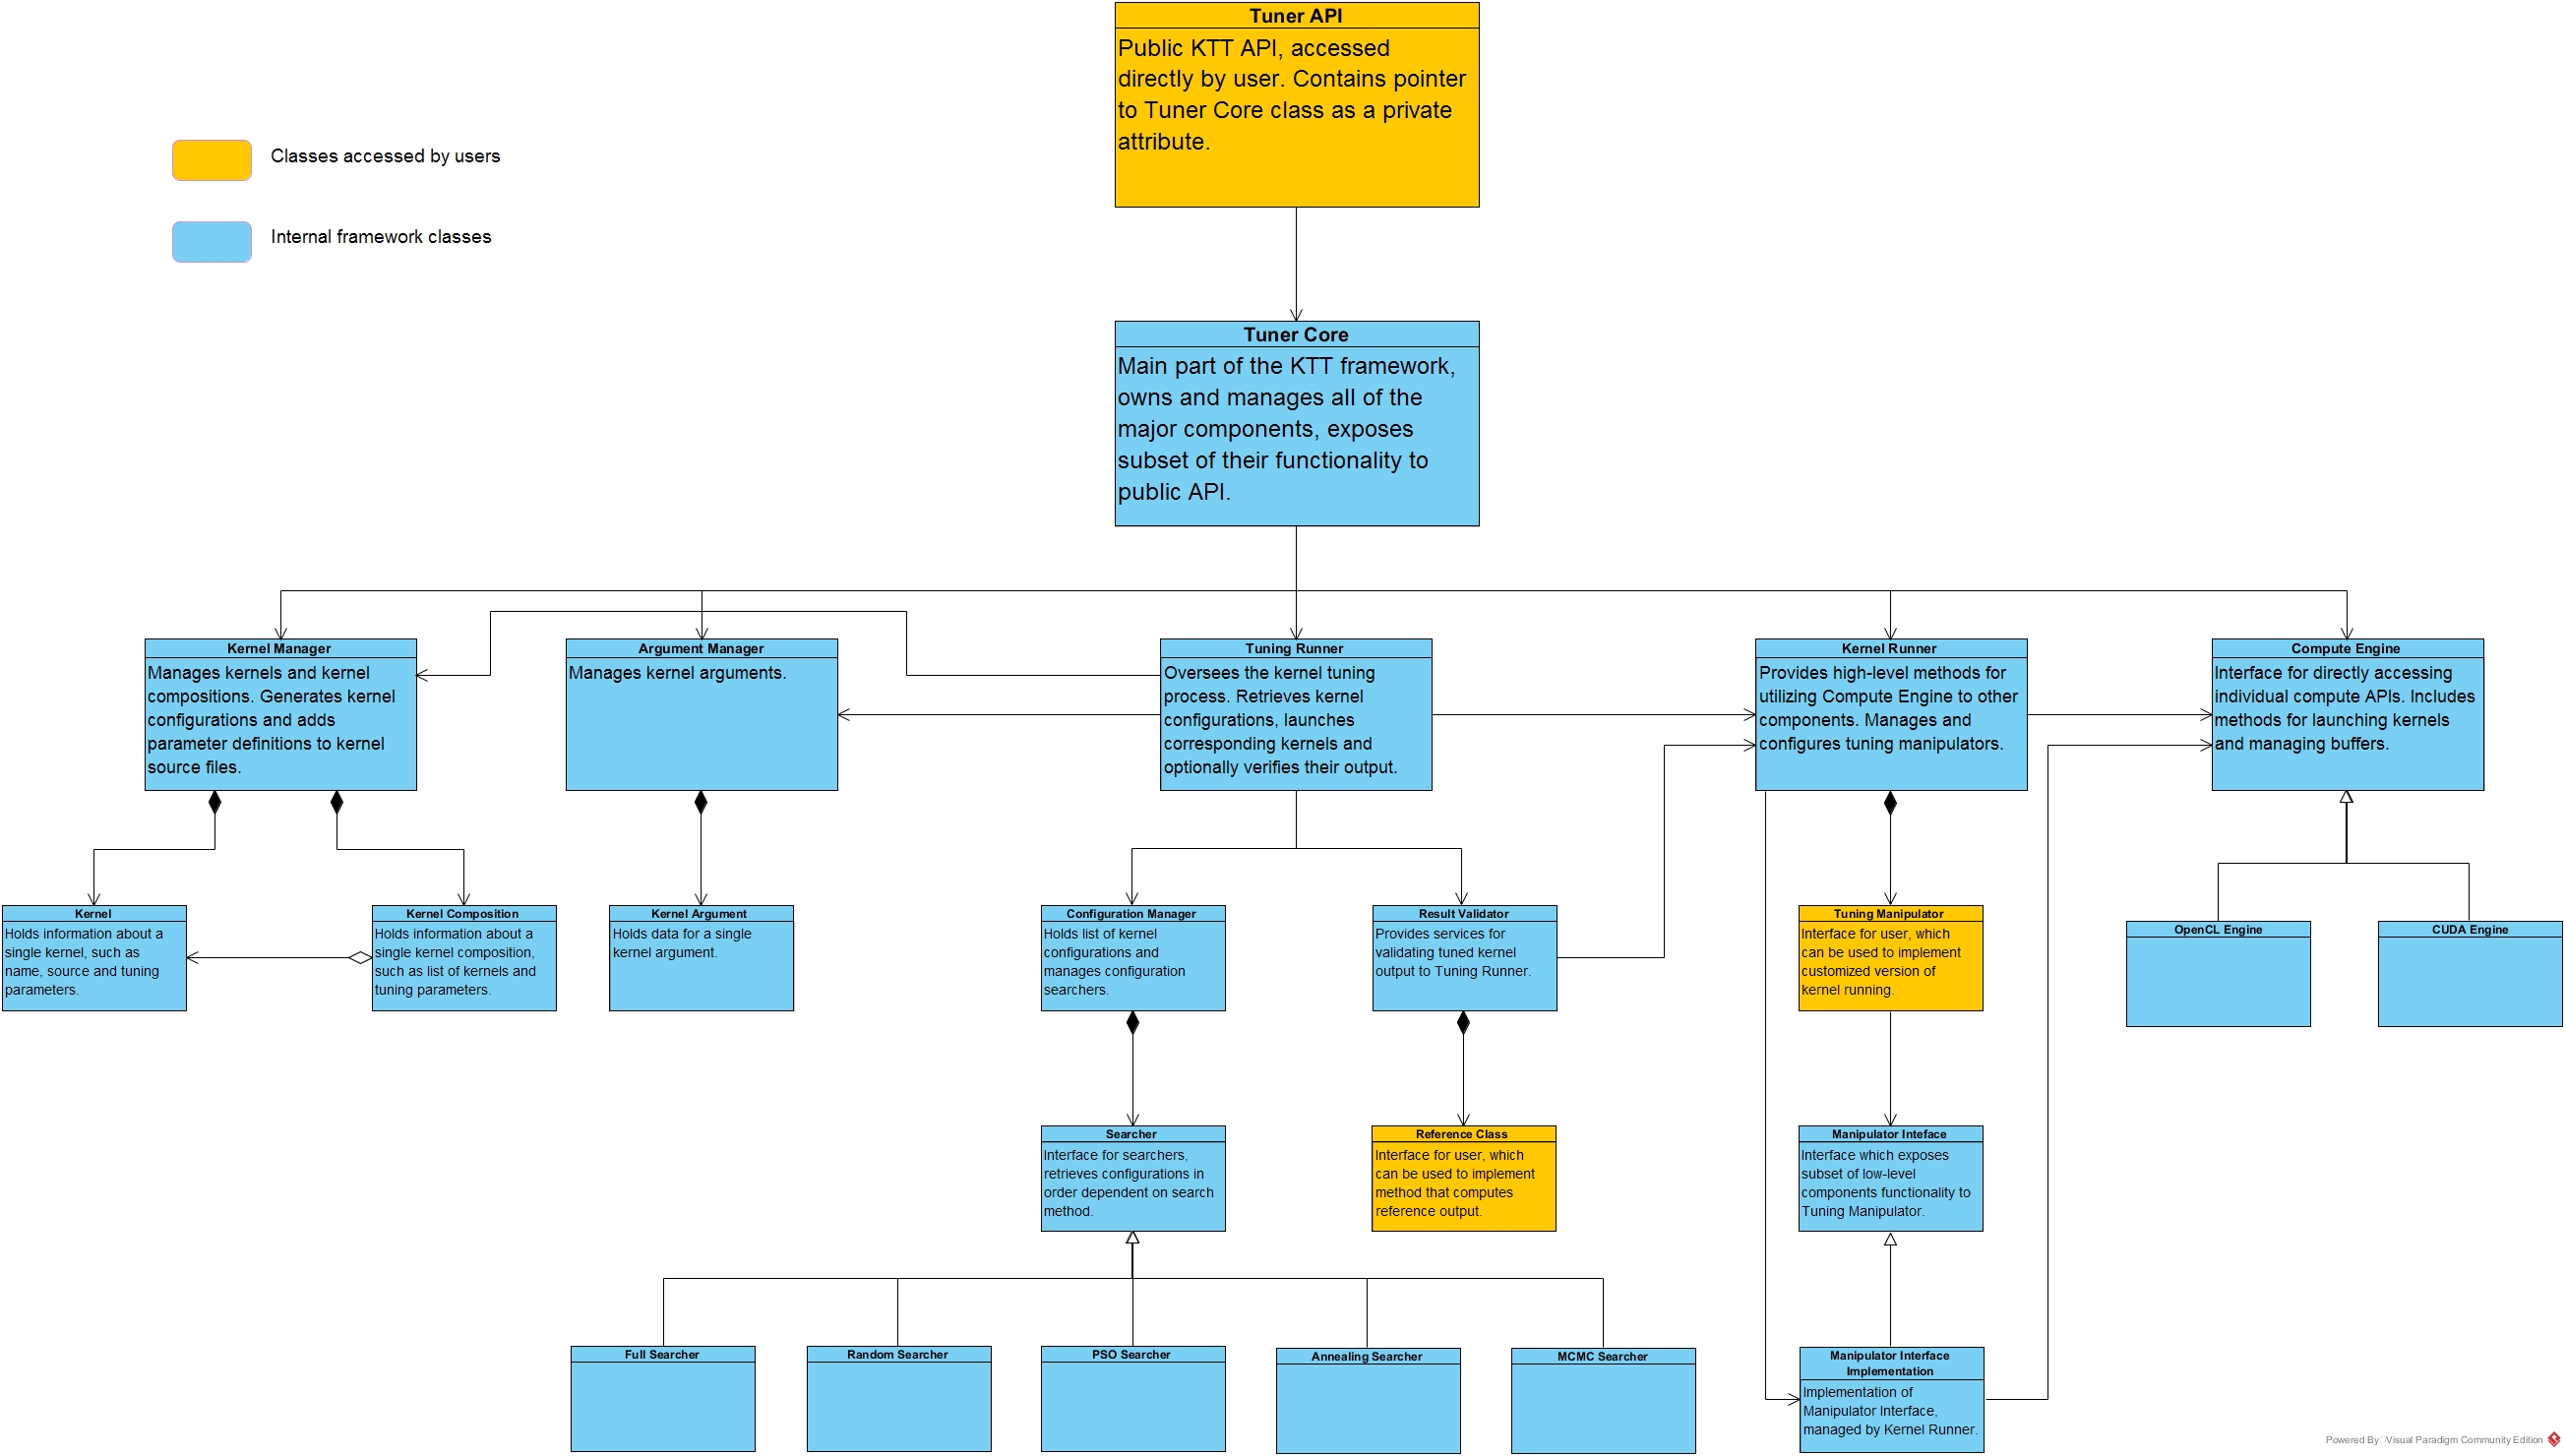
\includegraphics[width=250mm]{resources/ktt_class_diagram.jpg}  
    \end{adjustwidth}
    \caption{KTT class diagram. Note that two dependencies between kernel runner / kernel manager and kernel runner / argument manager were omitted
    in order to improve readability without severely impacting diagram accuracy.}
    \label{ktt-class-diagram}
\end{sidewaysfigure}
\clearpage

\section{Tuner and tuner core}
Tuner component represents the main part of public API. Its methods were described in chapter \ref{ktt-api}. In order to hide internal framework
components from users, it utilizes pointer to implementation idiom. The public header (.h) file contains only declaration of implementation class
(i.e., tuner core) and a pointer to its instance. However, the actual tuner core header with method definitions is directly included only in tuner
implementation (.cpp) file. This file is needed during compilation, but the built library can be then distributed with tuner header only. There is
no need to include internal headers for components such as tuner core, which makes upgrading to newer version of framework easier in certain situations
(e.g., if methods in tuner core are modified in newer version of the framework, but methods in tuner API remain the same, software which utilizes the
framework only needs to replace library file without recompilation).

Tuner core makes up the main internal part of the framework. It owns and manages several smaller components and exposes subset of their functionality
to public API. In some cases, it combines functionality of methods from multiple components into a single public API method.

\section{Kernel manager}
Primary task of a kernel manager is storage and management of kernels and kernel compositions. Other responsibilities include assigning unique handles for
new kernels and compositions, adding tuning parameter definitions to kernel source code and generating kernel configurations which are then used by other
components.

Configurations are generated recursively with parameters being processed one by one. The method which generates configurations contains a loop which
launches a new instance of the same method for each parameter value. The new instances then repeat the process for subsequent parameters until the
resulting configuration contains definitions of all parameters. When a configuration is complete, it is checked whether it satisfies all user-defined
constraints. Configurations which pass the check are then placed inside a shared vector container which is visible from all instances of recursively
called methods, invalid configurations are discarded. Kernel configurations also include global and local kernel thread sizes, which are updated when
a thread-modifying tuning parameter is processed. With multiple such parameters, the modification happens in the order of their addition.

Kernel compositions are components which contain references to all kernels that they include. Addition of tuning parameters works in a similar fashion
as for regular kernels, difference being that when a parameter is added to a composition, its definition is added to source codes of all utilized kernels.
If there is a kernel, which does not utilize certain parameter, the definition can be safely ignored. However, it is still possible to add thread-modifying
parameters which only affect thread sizes of a specific kernel inside a composition.

\section{Argument manager}
Argument manager stores and generates unique handles for kernel arguments. Arguments inside KTT can store elements with user-defined data types as well as
built-in data types. This is handled by storing the argument elements as raw data and converting to proper data type when needed (e.g., during result
validation). Restriction is that the used data type has to be trivially copyable\footnote{Trivially copyable data type cannot have user-defined
copy / move constructors, destructor or assignment operators and cannot contain virtual methods, which effectively makes it safe to copy with low-level
functions such as std::memcpy.}. However, this is not much of a problem because data which is copied into e.g., GPU memory should be trivially copyable
either way.

\section{Tuning runner, configuration manager and result validator}
Tuning runner and its two subcomponents -- configuration manager and result validator, oversee both offline and online tuning. During offline tuning,
result validator first computes reference output using reference class or kernel. Configurations generated by a kernel manager are then handed over to
a configuration manager which instantiates a searcher based on user-specified search method. Kernels or kernel compositions are then launched in a loop
using different configurations. The loop consists of the following steps:
\begin{enumerate}
    \item Tuning runner retrieves next configuration from configuration manager. Order of tested configurations depends on a searcher which is
    a subcomponent of configuration manager.
    \item Tuning runner launches a computation using previously retrieved configuration.
    \item When computation is finished, the output is compared with previously generated reference output.
    \item Computation duration is reported back to configuration manager, the duration can be utilized by searcher to optimize exploration of
    configuration space. Durations for failed computations or invalid results are reported as infinity.
\end{enumerate}
Once the loop finishes, tuning runner performs cleanup and the tuning results are stored for later retrieval.

Online tuning contains similar steps as offline tuning, except that it performs only single iteration of previously described loop per online tuning
method invocation. The other important difference is that if result validation is enabled, the reference output has to be recomputed for each
configuration as the output between launches of individual configurations may change. Since online tuning method can be launched more times than the
total number of available configurations, tuner always launches computation with the best found configuration after completing the exploration of
configuration space.

\section{Compute engine}
Compute engine serves as an interface for implementing support for multiple compute APIs into KTT framework. It abstracts relatively complicated
low-level compute API functions into smaller number of easier-to-use methods. It also provides automatic management of certain resources such as context,
command queues, kernels and events. Other framework components then do not need to utilize the specific compute API functions but rather use unified
compute engine interface. This simplifies addition of new compute APIs into KTT and makes it possible to support multiple APIs in a single version of
KTT library.

Compute engine interface declares several virtual methods which need to be implemented by inheriting class which provides support for specific compute
API. These include methods for running kernels, managing buffers, retrieving results, synchronizing command queues and querying for information about
platforms and devices.

\section{Kernel runner and manipulator interface}
Kernel runner provides simplified methods for using compute engine to higher-level components such as tuner core or tuning runner. It handles running of
kernels both with and without tuning manipulators. It also allows running of kernel compositions which always have to use tuning manipulator. Manipulators
for individual kernels and compositions are stored inside this component as well.

Motivation for developing tuning manipulator API was to allow users to have greater control over the process of running kernel computations.
For example, certain computations require running the same kernel multiple times in a loop, computing portion of the result directly in C++ code or
utilizing multiple kernels. The main KTT API alone does not allow for such functionality because it provides only high-level kernel running methods which
are easier to use but only support simpler use cases. In order to handle the complex scenarios, users would need to have access to more fine-grained
functionality, similar to what is offered by compute engine.

However, exposing compute engine methods to public API directly would be problematic for two reasons. Firstly, as KTT framework is further developed,
declarations of compute engine methods often change in order to support new functionality. This would force users to frequently update their code
during transitions to newer version of the framework. Secondly, significant number of compute engine methods are intended to be used together as a part
of single computation (e.g., uploading kernel arguments into buffers followed by launch of a kernel) and having these methods declared in the main API
along with the high-level methods would cause confusion.

Because of these reasons, tuning manipulator and the related component called manipulator interface were developed. Users can define a class which
inherits from tuning manipulator and consequently gain access to its methods which provide functionality similar to compute engine. Tuning manipulator
contains a private pointer to manipulator interface and internally calls its methods. Implementing class for the manipulator interface is a part of
kernel runner and has direct access to compute engine. When a kernel or a composition utilizing tuning manipulator is run, kernel runner sets the
manipulator interface pointer inside tuning manipulator to the implementing class and computation may then normally proceed. This way users have access
to functionality of internal framework components without a need to directly expose these components in public API. 

\chapter{Advanced KTT usage examples}
\label{ktt-advanced-usage}
This chapter presents several examples which utilize advanced features of KTT framework. These include utilization of tuning manipulator, kernel
compositions, online auto-tuning and integration of KTT into existing software. The examples were contributed to KTT framework by multiple authors.

\section{Reduction example with tuning manipulator}
This example demonstrates tuning of a kernel which performs summation of floating-point numbers contained in a single array. The reduction can be
computed inside a kernel. It is possible to either finish the entire computation in a single kernel invocation utilizing atomic instructions or
compute the result iteratively over multiple kernel launches. The second scenario requires usage of tuning manipulator.

The example is split into three figures -- Figure \ref{reduction-example-main} contains the main part of a host program. Tuning parameters and
constraints are defined in Figure \ref{reduction-example-parameters} and Figure \ref{reduction-example-manipulator} includes definition of a
manipulator.

Host program begins with initialization of data and kernel dimensions (lines 6-17), default NDRange size corresponds to a total number of elements
rounded up to the nearest higher multiple of 512, which is the largest possible work-group size that kernel in this example utilizes. The following
lines (19-27) contain initialization of tuner, addition of kernel and its arguments. Kernel output is validated using reference class (line 32).
Since result of the computation is only a single number, validation range is set to one (line 33). Tuning manipulator is added to tuner in a similar
fashion as a reference class (line 34). The manipulator in this example modifies certain kernel arguments whose ids are passed into its constructor.
The remaining code section (lines 36-37) contains start of a tuning process and printing of results.

Tuning parameters are defined in the second figure (lines 5-9). The first parameter controls size of a work-group, same as in simple example in
section \ref{ktt-simple-usage}. The next two parameters are used to control number of work-groups. Parameter "UNBOUNDED\_WG" controls whether number
of work-groups scales based on input size. If the scaling is disabled, then their number is controlled with parameter "WG\_NUM" whose values are set
to a multiple of available compute units. The number of compute units and several other device parameters can be retrieved through KTT API
(lines 2-3). Parameter "VECTOR\_SIZE" controls which vector data type is used for input buffer. This parameter also divides the global size because
more elements are processed by a single work-item when longer vector types are used. The last parameter determines whether the computation is done
in a single kernel execution or iterative kernel launches are utilized. The example also makes use of multiple parameter constraints (lines 11-16).
For example, the first constraint ensures that only one of the parameters which affect number of work-groups remains active inside a configuration.

Tuning manipulator is defined in the third figure. Apart from constructor, it contains definition of a method which performs the computation. First,
it retrieves information about current configuration (lines 6-9), including parameters and modified kernel dimensions. If "UNBOUNDED\_WG" parameter
is inactive, it sets NDRange size based on a value of "WG\_NUM" parameter (lines 10-12). The kernel is then launched (line 13) using the corresponding
global and local size. In case atomic operations are used, the computation is then finished and tuning manipulator ends. Otherwise kernel is launched
repeatedly in iterations log(n) times, input size shrinking by half in each iteration (lines 15-36). Because an output from one iteration is used as
an input in next iteration, the source and destination buffers keep getting swapped (line 22). As the input size continuously shrinks, NDRange size
and several kernel arguments have to be updated in each iteration (lines 23-28). Once the input size reaches 1, the computation is finished. One extra
iteration is sometimes performed in order to ensure that result is inside the original destination buffer.

\begin{figure}
\footnotesize
\begin{adjustwidth}{-1cm}{-1cm}
\begin{lstlisting}
int main(int argc, char** argv)
{
    // Initialize platform / device index and path to kernel file.
    ...
    
    const int n = 32 * 1024 * 1024;
    const int nAlloc = ((n + 16 - 1) / 16) * 16;
    std::vector<float> src(nAlloc, 0.0f);
    std::vector<float> dst(nAlloc, 0.0f);
    int nUp = ((n + 512 - 1) / 512) * 512;
    ktt::DimensionVector ndRangeDimensions(nUp);
    ktt::DimensionVector workGroupDimensions(1);
    
    for (int i = 0; i < n; i++)
    {
        src[i] = 1000.0f * ((float)rand()) / ((float)RAND_MAX);
    }
    
    ktt::Tuner tuner(platformIndex, deviceIndex);
    ktt::KernelId kernelId = tuner.addKernelFromFile(kernelFile, "reduce", ndRangeDimensions, workGroupDimensions);
    ktt::ArgumentId srcId = tuner.addArgumentVector(src, ktt::ReadWrite);
    ktt::ArgumentId dstId = tuner.addArgumentVector(dst, ktt::ReadWrite);
    ktt::ArgumentId nId = tuner.addArgumentScalar(n);
    int offset = 0;
    ktt::ArgumentId inOffsetId = tuner.addArgumentScalar(offset);
    ktt::ArgumentId outOffsetId = tuner.addArgumentScalar(offset);
    tuner.setKernelArguments(kernelId, std::vector<ktt::ArgumentId>{srcId, dstId, nId, inOffsetId, outOffsetId});
    
    // Definition of tuning parameters and constraints is in separate figure.
    ...
    
    tuner.setReferenceClass(kernelId, std::make_unique<ReferenceReduction>(src, dstId), std::vector<ktt::ArgumentId>{dstId});
    tuner.setValidationRange(dstId, 1);
    tuner.setTuningManipulator(kernelId, std::make_unique<TunableReduction>(srcId, dstId, nId, inOffsetId, outOffsetId));
    
    tuner.tuneKernel(kernelId);
    tuner.printResult(kernelId, "reduction_output.csv", ktt::PrintFormat::CSV);
    return 0;
}
\end{lstlisting}
\caption{Main part of the reduction host program.}
\label{reduction-example-main}
\end{adjustwidth}
\end{figure}

\begin{figure}
\footnotesize
\begin{adjustwidth}{-1cm}{-1cm}
\begin{lstlisting}
    ...
    const ktt::DeviceInfo di = tuner.getCurrentDeviceInfo();
    size_t cus = di.getMaxComputeUnits();
    
    tuner.addParameter(kernelId, "WORK_GROUP_SIZE_X", {32, 64, 128, 256, 512}, ktt::ModifierType::Local, ktt::ModifierAction::Multiply, ktt::ModifierDimension::X);
    tuner.addParameter(kernelId, "UNBOUNDED_WG", {0, 1});
    tuner.addParameter(kernelId, "WG_NUM", {0, cus, cus * 2, cus * 4, cus * 8, cus * 16});
    tuner.addParameter(kernelId, "VECTOR_SIZE", {1, 2, 4, 8, 16}, ktt::ModifierType::Global, ktt::ModifierAction::Divide, ktt::ModifierDimension::X);
    tuner.addParameter(kernelId, "USE_ATOMICS", {0, 1});
    
    auto persistConstraint = [](std::vector<size_t> v) {return (v[0] == 1 && v[1] == 0) || (v[0] == 0 && v[1] > 0);};
    tuner.addConstraint(kernelId, persistConstraint, {"UNBOUNDED_WG", "WG_NUM"});
    auto persistentAtomic = [](std::vector<size_t> v) {return (v[0] == 1) || (v[0] == 0 && v[1] == 1);};
    tuner.addConstraint(kernelId, persistentAtomic, {"UNBOUNDED_WG", "USE_ATOMICS"});
    auto unboundedWG = [](std::vector<size_t> v) {return (v[0] == 0 || v[1] >= 32);};
    tuner.addConstraint(kernelId, unboundedWG, {"UNBOUNDED_WG", "WORK_GROUP_SIZE_X"});
    ...
\end{lstlisting}
\caption{Definition of tuning parameters and constraints in reduction host program.}
\label{reduction-example-parameters}
\end{adjustwidth}
\end{figure}

\begin{figure}
\footnotesize
\begin{adjustwidth}{-1cm}{-1cm}
\begin{lstlisting}
class TunableReduction : public ktt::TuningManipulator {
public:
  // Constructor initializes private manipulator attributes.

  void launchComputation(const ktt::KernelId kernelId) override {
        ktt::DimensionVector globalSize = getCurrentGlobalSize(kernelId);
        ktt::DimensionVector myGlobalSize = globalSize;
        ktt::DimensionVector localSize = getCurrentLocalSize(kernelId);
        auto parameterValues = getCurrentConfiguration();
        if (getParameterValue("UNBOUNDED_WG", parameterValues) == 0) {
            myGlobalSize = ktt::DimensionVector(getParameterValue("WG_NUM", parameterValues) * localSize.getSizeX());
        }
        runKernel(kernelId, myGlobalSize, localSize);

        if (getParameterValue("USE_ATOMICS", parameterValues) == 0) {
            size_t n = globalSize.getSizeX() / localSize.getSizeX();
            size_t inOffset = 0, outOffset = n, iterations = 0;
            size_t vectorSize = getParameterValue("VECTOR_SIZE", parameterValues);
            size_t wgSize = localSize.getSizeX();

            while (n > 1 || iterations % 2 == 1) {
                swapKernelArguments(kernelId, srcId, dstId);
                myGlobalSize.setSizeX((n + vectorSize - 1) / vectorSize);
                myGlobalSize.setSizeX(((myGlobalSize.getSizeX() - 1) / wgSize + 1) * wgSize);
                if (myGlobalSize == localSize) outOffset = 0;
                updateArgumentScalar(nId, &n);
                updateArgumentScalar(outOffsetId, &outOffset);
                updateArgumentScalar(inOffsetId, &inOffset);

                runKernel(kernelId, myGlobalSize, localSize);
                n = (n + wgSize * vectorSize - 1) / (wgSize * vectorSize);
                inOffset = outOffset / vectorSize;
                outOffset += n;
                iterations++;
            }
        }
    }

private:
    // Attributes are ids of kernel arguments passed to manipulator constructor.
};
\end{lstlisting}
\caption{Tuning manipulator for reduction kernel.}
\label{reduction-example-manipulator}
\end{adjustwidth}
\end{figure}

\clearpage
\section{Sorting example with kernel compositions}
Todo...

\begin{figure}
\footnotesize
\begin{adjustwidth}{-1cm}{-1cm}
\begin{lstlisting}
int main(int argc, char** argv) {
    // Initialize platform / device index and path to kernel file.
    ...
    ktt::Tuner tuner(platformIndex, deviceIndex);
    std::vector<ktt::KernelId> kernelIds(3);
    const ktt::DimensionVector ndRangeDimensions(1);
    const ktt::DimensionVector workGroupDimensions(1);
    
    kernelIds[0] = tuner.addKernelFromFile(kernelFile, std::string("reduce"), ndRangeDimensions, workGroupDimensions);
    kernelIds[1] = tuner.addKernelFromFile(kernelFile, std::string("top_scan"), workGroupDimensions, workGroupDimensions);
    kernelIds[2] = tuner.addKernelFromFile(kernelFile, std::string("bottom_scan"), ndRangeDimensions, workGroupDimensions);
    
    // Addition of kernel arguments.
    ...
    ktt::KernelId compositionId = tuner.addComposition("sort", kernelIds, std::make_unique<TunableSort>(kernelIds, size, inId, outId, isumsId, sizeId, localMem1Id, localMem2Id, localMem3Id, numberOfGroupsId, shiftId));
    tuner.setCompositionKernelArguments(compositionId, kernelIds[0], std::vector<size_t>{inId, isumsId, sizeId, localMem1Id, shiftId});
    tuner.setCompositionKernelArguments(compositionId, kernelIds[1], std::vector<size_t>{isumsId, numberOfGroupsId, localMem2Id});
    tuner.setCompositionKernelArguments(compositionId, kernelIds[2], std::vector<size_t>{inId, isumsId, outId, sizeId, localMem3Id, shiftId});
    
    tuner.addParameter(compositionId, "FPVECTNUM", {4, 8, 16});
    tuner.addParameter(compositionId, "LOCAL_SIZE", {128, 256, 512});
    tuner.addParameter(compositionId, "GLOBAL_SIZE", {512, 1024, 2048, 4096, 8192, 16384, 32768});
    auto workGroupConstraint = [](std::vector<size_t> vector) {return vector.at(0) != 128 || vector.at(1) != 32768;};
    tuner.addConstraint(compositionId, workGroupConstraint, {"LOCAL_SIZE", "GLOBAL_SIZE"});
    
    tuner.setReferenceClass(compositionId, std::make_unique<ReferenceSort>(in), std::vector<ktt::ArgumentId>{outId});
    tuner.tuneKernel(compositionId);
    tuner.printResult(compositionId, std::string("sort_result.csv"), ktt::PrintFormat::CSV);
    return 0;
}
\end{lstlisting}
\caption{Sorting host program.}
\label{sort-example-main}
\end{adjustwidth}
\end{figure}

\begin{figure}
\footnotesize
\begin{adjustwidth}{-1cm}{-1cm}
\begin{lstlisting}
void launchComputation(const ktt::KernelId) override {
    const int radix_width = 4;
    std::vector<ktt::ParameterPair> parameterValues = getCurrentConfiguration();
    int localSize = (int)getParameterValue("LOCAL_SIZE", parameterValues);
    const ktt::DimensionVector workGroupDimensions(localSize);
    int globalSize = (int)getParameterValue("GLOBAL_SIZE", parameterValues);
    const ktt::DimensionVector ndRangeDimensions(globalSize);
    
    int numberOfGroups = globalSize / localSize;
    updateArgumentScalar(numberOfGroupsId, &numberOfGroups);
    updateArgumentLocal(localMem1Id, localSize);
    updateArgumentLocal(localMem2Id, 2 * localSize);
    updateArgumentLocal(localMem3Id, 2 * localSize);
    int isumsSize = (numberOfGroups * 16 * sizeof(unsigned int));
    std::vector<unsigned int> is(isumsSize);
    updateArgumentVector(isumsId, is.data(), isumsSize);
    
    bool inOutSwapped = false;
    for (int shift = 0; shift < sizeof(unsigned int) * 8; shift+=radix_width) {
        updateArgumentScalar(shiftId, &shift);
        bool even = ((shift / radix_width) % 2 == 0) ? true : false;
        if (even) {
            changeKernelArguments(kernelIds[0], {inId, isumsId, sizeId, localMem1Id, shiftId});
        } else {
            changeKernelArguments(kernelIds[0], {outId, isumsId, sizeId, localMem1Id, shiftId});
        }
        
        runKernel(kernelIds[0], ndRangeDimensions, workGroupDimensions);
        runKernel(kernelIds[1], workGroupDimensions, workGroupDimensions);
        runKernel(kernelIds[2], ndRangeDimensions, workGroupDimensions);
        
        swapKernelArguments(kernelIds[2], inId, outId);
        if (shift + radix_width < sizeof(unsigned int) * 8)
            inOutSwapped = !inOutSwapped;
    }
    if (inOutSwapped)
        copyArgumentVector(outId, inId, size);
}
\end{lstlisting}
\caption{Computation method inside tuning manipulator in sorting example.}
\label{sort-example-manipulator}
\end{adjustwidth}
\end{figure}

\section{Integrating KTT into software and online auto-tuning}
Todo...

\FloatBarrier

\chapter{Conclusion}
The framework developed as a part of this thesis contains all the functionality needed to fulfill the assignment. Certain features such as tuning
manipulators or possibility of online tuning are not yet supported by any other publicly available framework and KTT therefore offers improvements
over current state-of-the-art auto-tuning software. Furthermore, it was demonstrated that the stated features can be used in practice in scenarios
such as auto-tuning of non-trivial computations which utilize multiple kernels or integration into other software where it can be used to combine
online tuning with regular computation.

However, there is still a lot of room left for improvements and many ways in which the framework could be extended. It would be interesting to explore
viability of auto-tuning in area of graphics applications and shaders with addition of support for APIs such as Vulkan or OpenGL. Another improvement
could be made in the area of tuning for different input sizes since the tuner currently assumes that the input size does not change significantly during
exploration of configuration space. The exploration itself could use some additional improvements as well with support for more search optimization
techniques. It would be also useful to develop a tool which analyses the impact of individual tuning parameters and their combinations on performance on
specific devices or a tool for tuning results visualization.

%% Print full bibliography, use biber.exe on .bcf file to generate bibliography
\csname captions\languagename\endcsname
\makeatletter
\thesis@selectLocale{\thesis@locale}\makeatother
\printbibliography[heading=bibintoc]

\appendix
\chapter{Electronic attachment}
Electronic attachment for the thesis is available in Information System of Masaryk University. It contains the following materials:
\begin{itemize}
    \item thesis text in PDF format
    \item full source code for version 0.6 of KTT framework
    \item supplementary KTT framework materials such as API documentation, tutorials and example projects
\end{itemize}

\end{document}
